%  LaTeX support: latex@mdpi.com 
%  For support, please attach all files needed for compiling as well as the log file, and specify your operating system, LaTeX version, and LaTeX editor.

%=================================================================
\documentclass[journal,article,submit,pdftex,moreauthors]{Definitions/mdpi} 

% MDPI counters
\firstpage{1} 
\makeatletter \setcounter{page}{\@firstpage} \makeatother
\pubvolume{1}
\issuenum{1}
\articlenumber{0}
\pubyear{2025}
\copyrightyear{2025}
\datereceived{ } \daterevised{ } \dateaccepted{ } \datepublished{ } 
\hreflink{https://doi.org/}

% Custom macros
\newcommand{\vect}[1]{\boldsymbol{#1}}
\newcommand{\tr}{\operatorname{tr}}

% Title and metadata
\Title{Data-Driven Hyperelastic Constitutive Neural Network Model with Laplace Parameterization}
\TitleCitation{CLANN (Convex Laplace Artificial Neural Network)}

\newcommand{\orcidauthorA}{0000-0002-5860-4419}
\Author{Dits D. $^{1}$\orcidA{}, Ovsepyan A., Lyogkiy A., Salamatova V. }
\AuthorNames{Dits D., et al.}
\isAPAStyle{\AuthorCitation{Dits D., et al.}}{\isChicagoStyle{\AuthorCitation{Dits D., et al.}}{\AuthorCitation{Dits D., et al.}}}
\address{$^{1}$ \quad Affiliation; e-mail@e-mail.com}
\corres{Correspondence: e-mail@e-mail.com}

\abstract{This paper presents a mathematical description of CLANN (Convex Laplace Artificial Neural Network), a neural model for hyperelastic materials in nonlinear continuum mechanics. The model is built on hyperelasticity, convexity, and frame invariance. A Cholesky-based logarithmic parameterization of the right Cauchy--Green tensor ensures convexity and enables stable differentiation. An input convex neural network (ICNN) with nonnegative output weights defines a strictly convex stored-energy density. Second Piola--Kirchhoff stresses are obtained by differentiating the energy with respect to the strain measure via the chain rule, which guarantees thermodynamic consistency and objective, conservative stresses. We provide explicit 2D formulas for stresses and an analytic Hessian used in Newton's method, together with a training loss that augments data misfit with anchors at the undeformed state to enforce zero energy and zero stress. The convexity of the energy yields positive-definite tangent moduli and robust convergence, while the logarithmic parameterization handles large strains. The approach integrates efficiently with finite element solvers and recovers linear elasticity in the small-strain limit.}
\keyword{hyperelasticity; convex neural networks; continuum mechanics; thermodynamics; finite elements}

\begin{document}

% Introduction
\section{Introduction}
\section{Введение}

% Математические модели, способные предсказывать нелинейное механическое поведение мягких материалов при больших деформациях, требуются в широком спектре инженерных отраслей -- от полимерной промышленности, до робототехники и персонализированной медицины \cite{
% Mechanical characterization and FE modelling of a hyperelastic material
% Quantifying the uncertainty in a hyperelastic soft tissue model with stochastic parameters
% Control-oriented models for hyperelastic soft robots through differential geometry of curves
% }
% Основой таких моделей служит нелинейная теория упругости \cite{A Comparative Study of Several Material Models for Prediction of Hyperelastic Properties: Application to Silicone-Rubber and Soft Tissues}, где 
% зависимость тензора напряжений от переменных, характеризующих кинематику материала, описывается так называемыми определяющими соотношениями, или уравнениями состояния \cite{Nonlinear solid mechanics: a continuum approach for engineering science}. 
% При моделировании напряженно-деформированного состояния полимеров и биологических тканей широко распространены гиперупругие определяющие соотношения \cite{
% Hyperelastic structures: A review on the mechanics and biomechanics}.

% В гиперупругой постановке постулируется существование упругого потенциала $\psi$, зависящего от выбранной меры деформации, который полностью описывает механическое поведение материала. При этом он должен удовлетворять ряду требований: отражать материальную симметрию, не зависеть от выбранной системы отсчета, обладать свойствами поливыпуклости \cite{Convexity conditions and existence theorems in nonlinear elasticity}, что является достаточным условием существования решений краевых задач гиперупругости \cite{Mathematical elasticity: Three-dimensional elasticity
% Hyperelastic membrane modelling based on data-driven constitutive relations}.

% Для мягких материалов предложено множество гиперупругих моделей \cite{Hyperelastic energy densities for soft biological tissues: a review}, большинство из которых удовлетворяют требованиям к материальной симметрии, объективности и поливыпуклости благодаря инвариантному подходу. Это означает, что для выбранной меры деформации задается набор инвариантов, а упругий потенциал является функцией этих инвариантов. Обычной практикой является использование инвариантов правых/левых тензоров деформации Коши-Грина. Для изотропных материалов упругий потенциал может быть выражен как функция от трех инвариантов правого тензора деформации Коши-Грина $\psi = \psi_{vol}(J) + \psi_{iso}(I_1,I_2,I_3)$, где $J$ -- якобиан, выражающий изменение объема тела при деформации, $I_1, I_2, I_3$ -- инварианты правого тензора деформации Коши-Грина. 
% Дальнейшим расширением инвариантного подхода является введение так называемых псевдоинвариантов правого тензора Коши-Грина $I_4,...I_8$, позволяющих описывать классы трансверсально-изотропных и ортотропных материалов. \cite{Nonlinear solid mechanics: a continuum approach for engineering science}.
% %Для несжимаемого трансверсально-изотропного материала упругий потенциал задается как $\psi = \psi_{iso}(I_1,I_2,I_3) + \psi_{aniso}(I_4,I_5)$ .
% %, где $I_4 = \mathbf{a_0} (\mathbf{F}^{\mathrm{T}} \mathbf{F})\mathbf{a_0}$, $I_5 = \mathbf{a_0} (\mathbf{F}^{\mathrm{T}} \mathbf{F})^2 \mathbf{a_0}$ 
% Такой подход требует априорного задания упругого потенциала аналитической функцией с параметрами, которые определяются из экспериментальных данных. Основными недостатками этого подхода являются неединственность оптимального набора параметров модели, отсутствие у инвариантов прямого физического смысла в терминах деформации \cite{On the use of the upper triangular (or QR) decomposition for developing constitutive equations for Green-elastic materials} с вытекающим из этого требованием к натурному эксперименту, а именно, достижение однородности деформаций и напряжений при механическом исследовании тестировании материала, субъективность выбора формы потенциала из   множества построенных экспертами моделей \cite{Interpretable data-driven modeling of hyperelastic membranes}.

% В некоторой степени, эти недостатки устраняют конструированием наилучшей гиперупругой модели регрессионными методами из набора априорно заданных мономов на основе инвариантов \cite{A new family of Constitutive Artificial Neural Networks towards automated model discovery}, или редукцией обобщенных моделей на основе информационного анализа экспериментальных данных \cite{On the AIC-based model reduction for the general Holzapfel–Ogden myocardial constitutive law}. В совокупности с полнополевыми методами оценки экспериментальных деформаций (цифровая корреляция избражений DIC \cite{High-speed 3D digital image correlation vibration measurement: Recent advancements and noted limitations}), методами виртуальных полей VFM \cite{VFM} и inverse FE \cite{NN-Euclid}, это становится мощным инструментом моделирования механики материалов в рамках гиперупругости. Однако, такие подходы остаются феноменологическими и все так же требуют экспертный выбор модели.

% Важное преимущество гиперупругой постановки состоит в том, что она не требует знания аналитического вида упругого потенциала. Для задания определяющих соотношений в случае гиперупругого материала, достаточно знать производные упругого потенциала по выбранной мере деформации, так называемые функции отклика \cite{Nonlinear solid mechanics: a continuum approach for engineering science}. С применением полнополевых методов оценки экспериментальных деформаций DIC и напряжений \cite{Numerical_study_of_stress_estimation_methods_for_membrane_inflation
% In vitro analysis of localized aneurysm rupture}, функции отклика могут быть построены напрямую на основе экспериментальных данных, полученных при тестировании материала в широком диапазоне различных режимов деформации. Это стимулирует исследование подходов к построению гиперупругих моделей, основанных на данных \cite{Data-driven computational mechanics}. 

% В работах \cite{Interpretable data-driven modeling of hyperelastic membranes
% Data-Driven Anisotropic Biomembrane Simulation Based on the Laplace Stretch} предлагается метод прямого моделирования механики изотропных и анизотропных материалов, основанного на данных, с использованием функций отклика, основанных на физически интерпретируемой мере деформации Лапласа\cite{On the use of the upper triangular (or QR) decomposition for developing constitutive equations for Green-elastic materials
% Laplace stretch: Eulerian and Lagrangian formulations}, в котором обходят проблемы инвариантной формулировки гиперупругой модели, напрямую строя функции отклика на основе экспериментальных данных. При этом не требуются какие-либо предварительные знания о симметрии материала. Совокупность функций отклика формирует таблично-заданное определяющее соотношение.
% Нелинейная система алгебраических уравнений для виртуального квазистатического растяжения и раздутия материалов в этих случаях решается простым методом релаксации, где метод интерполяции обратного взвешенного расстояния находит требуемые значения функций отклика на каждой итерации в любой точке пространства деформаций Лапласа. 
% Ограничениями такого подхода являются требования к "богатству" данных и невозможность применения градиентных методов решения нелинейных систем алгебраических уравнений в силу дискретности таблично-заданного определяющего соотношения.

% Параллельно с этим развиваются физически-информированные нейросетевые подходы, в частности выпуклые по входу нейронные сети (ICNN) \cite{Input Convex Neural Networks}, позволяющие "вшивать" в архитектуру сети объективность, монотонность и выпуклость по входу, являясь прокси к поливыпуклости, тем самым удовлетворяя требованиям к гиперупругим потенциалам \cite{Benchmarking physics-informed frameworks for data-driven hyperelasticity}. В работе \cite{NEURAL NETWORKS MEET ANISOTROPIC HYPERELASTICITY: A FRAMEWORK BASED ON GENERALIZED STRUCTURE TENSORS AND ISOTROPIC TENSOR FUNCTIONS} показана инвариантная архитектура физически-информированной нейронной сети, совместимая с конечно-элементными пакетами. Несмотря на интерпретируемость и термодинамическую корректность, архитектура сети включает в себя набор предположений -- обобщенных структурных тензоров \cite{Ebbing Phd}, что фактически фиксирует класс симметрии материала.

% В рамках данной работы мы предлагаем подход, который объединяет преимущества представления гиперупругой модели таблично-заданным определяющим соотношением в мерах деформаций Лапласа \cite{Data-Driven Anisotropic Biomembrane Simulation Based on the Laplace Stretch} и физически-информированных нейронных сетей \cite{Input Convex Neural Networks}, удовлетворяющих требованиям к гиперупругим моделям механики материалов. Мы формулируем термодинамически корректный, объективный по построению, выпуклый по входу, и не требующий знаний о симметрии материала гиперупругий потенциал, %%в котором анизотропия восстанавливается непосредственно из данных.
% Гладкость аппроксимации обеспечивает совместимость с градиентными методами решения систем нелинейных алгебраических уравнений. В сравнении с таблично-заданными определяющими соотношениями, CLaNN снимает ограничения, связанные с дискретностью аппроксимации, сохраняя интерпретируемость мер деформации и повышая устойчивость экстраполяции.

\paragraph{Область применимости и ограничения}
квазистатика, мембранная постановка, 

\paragraph{Организация статьи}




% Kinematics
\section{Kinematics}
\section{Kinematics}
\textbf{Basic relations}

We consider the equilibrium of a thin incompressible hyperelastic membrane of thickness $H$ under
prescribed loads.
The membrane deformation is characterized by the deformation of its midsurface.
Let \(\vect{X}\) and \(\vect{x}\) denote point positions,
in the corresponding bases \(\vect{E}_{\alpha}\) and \(\vect{e}_{\alpha}\),
in the reference (undeformed) \(\Omega_0 \subset \mathbb{R}^2\) and current (deformed) \(\Omega_t \subset \mathbb{R}^2\)
configurations of the membrane surface, respectively.
The deformation is defined by the mapping \(\vect{x} = \vect{x}(\vect{X})\),
the surface deformation gradient is \(\mathbb{F} = \vect{e}_{\alpha}\otimes\vect{E}^{\alpha}\),
and the right Cauchy–Green tensor is \(\mathbb C = C_{\alpha\beta} \,\vect{e}_{\alpha} \otimes \vect{e}_{\beta} = \mathbb F^{\top} \mathbb F\).
To define the strain measure we use the Laplace measure \(\vect{\xi} = (\xi_1 , \xi_2 , \xi_3)^T\) \cite{xi2023},
which may be computed in two equivalent ways:
either via the QR decomposition of the deformation gradient \(\mathbb F = \vect Q \vect R\) with \(\tilde{\mathbb F} = \vect R\),
or via the Cholesky factorization of the right Cauchy–Green tensor \(\mathbb C = \tilde{\mathbb F}^{\top}\tilde{\mathbb F}\) (Appendix \ref{app:cholesky}).
In this case the hyperelastic strain energy is a function of the Laplace strain, \(\psi = \psi(\vect{\xi})\).


\textbf{Laplace strain measure}
In two dimensions we introduce
\begin{equation}
\xi_1 = \ln(\tilde f_{11}),\quad \xi_2 = \ln(\tilde f_{22}),\quad \xi_3 = \frac{\tilde f_{12}}{\tilde f_{11}}, 
\quad \tilde{\mathbb F} = \tilde f_{\alpha\beta} \; \vect{e}_{\alpha} \otimes \vect{e}_{\beta}.
\label{eq:laplace_coords}
\end{equation}




% Stress and consistency
\section{Stress and Thermodynamic Consistency}
\section{Напряжение и термодинамическая корректность}

В качестве меры напряжения образца мы используем \textbf{второй тензор напряжений Пиолы-Кирхгофа}, который вычисляется по цепному правилу дифференцированием энергии \(\psi\) 
по правому тензору деформации Коши-Грина \(\vect C\):

\begin{equation}
  \mathbf{S} \;=\; 2\,\frac{\partial \psi}{\partial \mathbf{C}}
  \;=\; 2\,\frac{\partial \psi}{\partial \boldsymbol\xi} \cdot \frac{\partial \boldsymbol\xi}{\partial \mathbf{C}}
  \;=\; 2\,\mathbf{r}(\boldsymbol\xi)\cdot\frac{\partial \boldsymbol\xi}{\partial \mathbf{C}},
  \qquad \mathbf{r}:=\frac{\partial \psi}{\partial \boldsymbol\xi}.
  \label{eq:chain-rule}
\end{equation}
Вектор $\frac{\partial \boldsymbol\xi}{\partial \mathbf{C}}$ называют базисом, он является известным \colorbox{yellow}{В смысле расхожим, или известным из экспериментальных данных?} аналитическим выражением, зависящим от выбранной меры деформации; $\vect{r} = (r_1, r_2, r_3)$ -- функцией отклика, которая является итоговым \textit{искомым} в процессе обучения \textit{data-driven} определяющего соотношения.   

Такое построение имеет ключевые следствия:
\newline
\textit{Объективность:} $\psi(\mathbf{C})=\psi(\mathbf{Q}^\top\mathbf{C}\mathbf{Q})$ для любой ортогональной $\mathbf{Q}$, а значит и $\mathbf{S}$ инвариантен к поворотам.
\newline
\textit{Симметрия напряжений:} $\mathbf{S}=\mathbf{S}^\top$ вследствие симметрии $\mathbf{C}$ и корректного применения цепного правила.
\newline
\textit{Термодинамическая корректность:} равенство \eqref{eq:chain-rule} является следствием неравенства Клаузиуса-Дюгема 
$\mathcal{D} = \mathbf{S} : \dot{\mathbf{C}} - \dot{\psi}(\mathbf{C}) \geq 0$, 
выражающее второе начало термодинамики для механических процессов \cite{truesdell1984historical,truesdell2004nonlinear}.
% \begin{itemize}
%   \item \textbf{Объективность:} $\psi(\mathbf{C})=\psi(\mathbf{Q}^\top\mathbf{C}\mathbf{Q})$ для любой ортогональной $\mathbf{Q}$, а значит и $\mathbf{S}$ инвариантен к поворотам.
%   \item \textbf{Симметрия напряжений:} $\mathbf{S}=\mathbf{S}^\top$ вследствие симметрии $\mathbf{C}$ и корректного применения цепного правила.
%   \item \textbf{Термодинамическая корректность:} равенство \eqref{eq:chain-rule} является следствием неравенства Клаузиуса-Дюгема 
%   $\mathcal{D} = \mathbf{S} : \dot{\mathbf{C}} - \dot{\psi}(\mathbf{C}) \geq 0$, 
%   выражающее второе начало термодинамики для механических процессов \cite{truesdell1984historical,truesdell2004nonlinear}.
% \end{itemize}

% \textbf{Связь тензора Лапласа и второго тензора напряжений Пиолы-Кирхгофа}

 % Необходимо установить связь деформации Лапласа $\vect{\xie}$ и второго тензора напряжений Пиолы-Кирхгофа $\vect{S}$. Применяя цепное правило дифференцирования к выражению \eqref{eq:chain-rule} и используя меру деформации Лапласа,

Расписав покомпонентно уравнение \eqref{eq:chain-rule} и подставив туда известный базис $\frac{\partial \boldsymbol\xi}{\partial \mathbf{C}}$, получаем аналитические выражения для компонент второго тензора напряжений Пиолы-Кирхгофа в двумерном случае:

\begin{equation}
\begin{aligned}
  S_{11} &= e^{-2\xi_1}\big(r_1-2\xi_3 r_3\big) + e^{-2\xi_2} r_2\,\xi_3^2,\\
  S_{22} &= e^{-2\xi_2} r_2,\\
  S_{12} &= -e^{-2\xi_2} r_2\,\xi_3 + e^{-2\xi_1} r_3,
\end{aligned}
\label{eq:stress_components_2d}
\end{equation}
% $r_1, r_2, r_3$ — компоненты функции отклика $\mathbf{r} = \frac{\partial \psi}{\partial \boldsymbol\xi}$.

\textbf{Фундаментальные ограничения\colorbox{yellow}{чего? на что? Лучше первым абзацем архитектуры, как требования к гиперупругому потенциалу}}

В соответствии с принципами термодинамики и механики сплошных сред, 
гиперупругая модель $\psi$ должна удовлетворять ряду фундаментальных ограничений, обеспечивающих физическую корректность и 
материальную устойчивость:
\newline
\textit{Неотрицательность} исключает отрицательную энергию деформации
  \begin{equation}
    \psi(\vect{\xi}) \ge 0\quad \forall\,\vect{\xi}\in\mathbb{R}^3.
    \label{eq:non_negativity}
  \end{equation}
  % Это 
\newline  
 \textit{Нулевые значения для $\psi$ и $\vect S$ в естественном состоянии} означают, что недеформированное (начальное) состояние среды не имеет остаточных напряжений
  \begin{equation}
    \psi(\vect 0)=0,\qquad \vect S(\vect I)=\vect 0,
    \label{eq:natural_state_stress}
  \end{equation}
\newline
  \textit{Бесконечный рост (коэрцитивность)}. Неограниченный рост меры деформации физически недостижим при конечной работе \colorbox{yellow}{не совсем понятно, уместно ли говорить про $J\to\infty$ для случая несжимаемой мембраны}
  \begin{equation}
    \psi(\vect{\xi}) \to \infty\ \text{при}\ \lVert\vect{\xi}\rVert\to\infty,\qquad
    \vect{S} \to \infty\ \text{при}\ J\to\infty \text{ или } J\to 0^{+},\qquad
    J=\det\vect F,
    \label{eq:energy_constraints}
  \end{equation}
  % Это обеспечивает коэрцивность: крайние объёмные деформации ($J\to\infty$, $J\to 0^{+}$) и неограниченный рост меры деформации физически недостижимы при конечной работе.

Свойства \eqref{eq:non_negativity} -- \eqref{eq:energy_constraints} принято записывать через градиент деформации \(\vect{F}\) и правый тензор деформации Коши-Грина \(\vect{C}\) 
\cite{antman2005nonlin,green1839laws,kirchhoff1850gleichgewicht}, но они эквивалентны и для меры деформации Лапласа \(\vect{\xi}\).

% Свойства \eqref{eq:non_negativity} -- \eqref{eq:energy_constraints} 




% Architecture
\section{CLANN architecture and its derivatives}
\section{Архитектура CLaNN и её производные}

В рамках предложенного под  хода CLaNN (Convex Laplace Neural Network)
энергия деформации \(\psi(\vect{\xi})\) с мерой деформации Лапласа аппроксимириуется посредством 
выпуклой по входу нейронной сетью (Input Convex Neural Network, ICNN) \cite{icnn2017}
и вычисления 2 тензора напряжения Пиолы-Кирхгофа \(\vect{S}\). 

\textbf{Обобщенная архитектура ICNN}

ICNN представляет собой класс нейронных сетей, гарантирующих выпуклость выходной функции относительно входных переменных. 
В нашем случае, функция энергии деформации $\psi: \mathbb{R}^3 \rightarrow \mathbb{R}$ называется выпуклой, 
если $\forall \vect{\xi}_1, \vect{\xi}_2 \in \mathbb{R}^3$ и $\lambda \in [0,1]$ выполняется неравенство Йенсена:
\begin{equation}
\psi(\lambda \vect{\xi}_1 + (1-\lambda) \vect{\xi}_2) \leq \lambda \psi(\vect{\xi}_1) + (1-\lambda) \psi(\vect{\xi}_2).
\label{eq:convexity_definition}
\end{equation}

Ключевые условия ICNN \cite{icnn2017}: 
(i) поэлементно выпуклая, монотонно неубывающая активация $\varphi$; 
(ii) $\mathbf{W}_z^{(\ell)}\!\ge\!0$ для всех слоёв 
(только на связях $z\!\to\!z$; $\mathbf{W}_x^{(\ell)}$, $\mathbf{b}^{(\ell)}$ без ограничений по знаку); 
(iii) каждый слой имеет прямую аффинную связь с входом 
$\boldsymbol{\xi}$: $z^{(\ell+1)}=\varphi\!\big(\mathbf{W}_z^{(\ell)}z^{(\ell)}+\mathbf{W}_x^{(\ell)}\boldsymbol{\xi}+\mathbf{b}^{(\ell)}\big)$; 
(iv) скалярный выход как $a^{\top} z^{(L)}+c$ с $a\!\ge\!0$ (или ещё один слой $\varphi$).

\textbf{Шаг 1. Однослойный ICNN и выбор активации.}
Рассмотрим однослойный вариант ICNN (с одним скрытым слоем) для аппроксимации $\psi(\boldsymbol{\xi})$:
\begin{equation}
  s = \mathbf{W}_1 \,\boldsymbol{\xi} + \mathbf{b}_1,\qquad
  z = \varphi_{\beta}(s),\qquad
  \tilde{\psi} = \mathbf{W}_2^{\top} z + b_2,\qquad \mathbf{W}_2 \ge 0.
  \label{eq:icnn_onelayer}
\end{equation}

\begin{equation}
  \varphi_{\beta}(x) = \frac{\operatorname{softplus}(\beta x)}{\beta},
  \label{eq:softplus_activation}
\end{equation}

Здесь $\varphi_{\beta}$ — выпуклая неубывающая функция активации \cite{dugas2001incorporating}, 
которая гладко аппроксимирует ReLU и при конечных $\beta$ является строго выпуклой; $\varphi_{\infty}(x)=\max(0,x)$.
Условие $\mathbf{W}_2\!\ge 0$ сохраняет выпуклость линейной комбинации. 
Размерности: $\mathbf{W}_1\!\in\mathbb{R}^{h\times 3}$, $\mathbf{b}_1\!\in\mathbb{R}^{h}$, 
$\mathbf{W}_2\!\in\mathbb{R}^{h}_{\ge 0}$, $h$ — размерность скрытого слоя.

\textbf{Шаг 2. Центрирование энергии $\psi$ в естественном состоянии.}
Для выполнения условия $\psi(\mathbf{0})=0$ центрируем энергию, 
вычитая значение нелинейной части при $\boldsymbol{\xi}=\mathbf{0}$:
\begin{equation}
  z_0 = \varphi_{\beta}(\mathbf{b}_1),\qquad
  \psi(\boldsymbol{\xi}) = \mathbf{W}_2^{\top}\big(z - z_0\big),\qquad (b_2 \equiv 0).
  \label{eq:center_psi}
\end{equation}
Тогда $\psi(\mathbf{0})=0$. Поскольку $z_0$ не зависит от $\boldsymbol{\xi}$, 
градиент $\partial\psi/\partial\boldsymbol{\xi}$ и гессиан $\partial^2\psi/\partial\boldsymbol{\xi}^2$ 
совпадают с таковыми для $\tilde{\psi}$, сохраняя выпуклость и гладкость.

\textbf{Шаг 3. Центрирование отклика $\mathbf{r}$ в естественной конфигурации.}
Для выполнения условия $\vect S(\vect I)=\vect 0$ обнулим линейный отклик в точке 
$\boldsymbol{\xi}=\mathbf{0}$:
\begin{equation}
  \mathbf{r}_0 := \frac{\partial \psi}{\partial \boldsymbol{\xi}}\bigg|_{\boldsymbol{\xi}=\mathbf{0}},\qquad
  \psi_{\mathrm{phys}}(\boldsymbol{\xi}) = \psi(\boldsymbol{\xi}) - \mathbf{r}_0^{\top}\boldsymbol{\xi}.
  \label{eq:phys_energy}
\end{equation}

Тогда $\psi_{\mathrm{phys}}(\mathbf{0})=0$ и $\mathbf{r}(\mathbf{0})=\mathbf{0}$, 
а по цепному правилу \eqref{eq:chain-rule} получаем $\mathbf{S}(\mathbf{I})=\mathbf{0}$. 
Вычитание линейного члена не меняет гессиан и сохраняет выпуклость. 
Так как $\mathbf{r}(\mathbf{0})=\mathbf{0}$, точка $\boldsymbol{\xi}=\mathbf{0}$ является минимумом 
$\psi_{\mathrm{phys}}$, и значит $\psi_{\mathrm{phys}}\ge 0$.

После получения $\psi_{\mathrm{phys}}$ автоматически вычисляются 
$\partial\psi/\partial\boldsymbol{\xi}$ средствами autodiff, реализованными в современных библиотеках для машинного обучения 
\cite{pytorch2019}, \cite{tensorflow2016}, \cite{jax2018}, 
после чего тензор напряжений $\mathbf{S}$ находится по формуле \eqref{eq:stress_components_2d} с 
использованием связи $\psi(\vect C)=\psi\big(\boldsymbol{\xi}(\vect C)\big)$.

Центрирование $\psi_{\mathrm{phys}}$ и $\mathbf{r}$ в естественном состоянии 
дает возможность гарантирования выполнения \eqref{eq:natural_state_stress} и
позволяет избежать дополнительных ограничений на параметры сети

% (заменено на TikZ-схему в рис.~\ref{fig:clann_arc})

\textbf{Аналитические выражения для производных энергии}

\textbf{Градиент энергии деформации}

Аналитическое дифференцирование функции энергии по переменным \(\xi\) даёт выражение для градиента:

\begin{equation}
 \vect{r} = \nabla_\xi \psi_{\mathrm{phys}} = \vect W_1^T \left( \vect W_2 \odot \sigma(\beta (\vect W_1 \vect \xi + \vect b_1)) \right) - \vect r_0,
\label{eq:energy_gradient}
\end{equation}
где $\sigma(x) = \frac{1}{1 + e^{-x}}$ - сигмоида, 
а операция $\odot$ обозначает поэлементное произведение (Hadamard product). 
Данное выражение демонстрирует, что градиент энергии является линейной комбинацией строк матрицы $\vect W_1^T$ с весами, 
определяемыми произведением выходных весов $\vect W_2$ и значений функции активации $\sigma(\beta (\vect W_1 \vect\xi + \vect b_1))$.

\textbf{Гессиан энергии деформации}

Вторые производные энергии по переменным \(\xi\) определяют гессиан, который имеет следующую аналитическую форму:

\begin{equation}
 H_{ij} = \sum_h \sigma'_h\,W_{2,h}\,W_{h,i}W_{h,j},
\label{eq:energy_hessian}
\end{equation}

где $\sigma' = \beta\,\sigma(1-\sigma)$ - производная сигмоиды, 
$\sigma=\operatorname{sigmoid}(\beta s)$, а $s=\vect W_1\xi+\vect b_1$.

\textbf{Материальная устойчивость и положительная определённость}

Из строгой выпуклости \(\psi(\xi)\) следует положительная определённость гессиана:
\begin{equation}
 \vect H = \frac{\partial^2\psi}{\partial\xi^2} > 0,
\label{eq:positive_hessian}
\end{equation}
что обеспечивает положительную определённость касательных модулей упругости 
$\mathbb{C} = \partial^2\psi/\partial\vect C^2$ через цепное правило дифференцирования. 
Это свойство важно для численной стабильности конечно-элементных расчётов, 
поскольку на практике улучшает сходимость метода Ньютона и отсутствие сингулярностей в матрице жёсткости.

% \begin{figure}[H]
%   \centering
%   \resizebox{\textwidth}{!}{% ===== CLaNN: однослойная ICNN (наглядная архитектура) =====
\begin{tikzpicture}[
  font=\small, node distance=9mm and 14mm, >={Latex},
  box/.style={draw, rounded corners, align=center, minimum height=7mm, inner sep=2mm},
  block/.style={box, fill=green!6, text width=44mm},
  pin/.style={circle, draw, minimum size=6mm, fill=white},
  neur0/.style={circle, draw, minimum size=6mm, fill=white},
  neur/.style={circle, draw, minimum size=6mm, fill=white},
  title/.style={font=\bfseries},
  every fit/.style={draw, rounded corners, inner sep=3mm}
]

% Входы (лог‑лапласовы координаты)
\node[pin] (x1) {$\xi_1$};
\node[pin, below=6mm of x1] (x2) {$\xi_2$};
\node[pin, below=6mm of x2] (x3) {$\xi_3$};

% Аффинная проекция
\node[neur0, right=14mm of x1, yshift=12mm] (h11) {};
\node[neur0, right=14mm of x1] (h12) {};
\node[neur0, right=14mm of x1, yshift=-12mm] (h13) {};
\node[align=center, right=14mm of x1, yshift=-22mm] (vdots0) {$\vdots$};
\node[neur0, right=14mm of x1, yshift=-34mm] (h14) {};
\draw[->] (x1) -- (h11.west);
\draw[->] (x2) -- (h11.west);
\draw[->] (x3) -- (h11.west);
\draw[->] (x1) -- (h12.west);
\draw[->] (x2) -- (h12.west);
\draw[->] (x3) -- (h12.west);
\draw[->] (x1) -- (h13.west);
\draw[->] (x2) -- (h13.west);
\draw[->] (x3) -- (h13.west);
\draw[->] (x1) -- (h14.west);
\draw[->] (x2) -- (h14.west);
\draw[->] (x3) -- (h14.west);
% \node[block, above=2mm of h11, text width=36mm] (aff) {$s = W_1\,\xi + b_1$};
\node[block, above=2mm of h11, text width=60mm, inner sep=3mm] (soft) {$z_i = \mathrm{softplus}(\beta (W_1\,\xi + b_1))/\beta$};

% % Скрытый слой (softplus): три нейрона, троеточие и ещё один
% \node[neur, right=14mm of h12, yshift=12mm] (h1) {};
% \node[neur, right=14mm of h12] (h2) {};
% \node[neur, right=14mm of h12, yshift=-12mm] (h3) {};
% \node[align=center, right=14mm of h12, yshift=-22mm] (vdots1) {$\vdots$};
% \node[neur, right=14mm of h12, yshift=-34mm] (h4) {};
% \draw[->] (h11.east) -- (h1.west);
% \draw[->] (h12.east) -- (h2.west);
% \draw[->] (h13.east) -- (h3.west);
% \draw[->] (h14.east) -- (h4.west);
% % Блок активации над нейронами
% \node[block, above=2mm of h1, text width=36mm] (soft) {$z_i = \mathrm{softplus}(\beta (W_1\,\xi + b_1)/\beta$};

% Линейный выход (неотрицательные веса)
\node[block, right=22mm of h12, text width=42mm] (readout) {$\psi(\boldsymbol{\xi}) = \mathbf{W}_2^{\top}\big(z - z_0\big) - \mathbf{r}_0^{\top}\boldsymbol{\xi}$};
\draw[->] (h11.east) -- (readout.west);
\draw[->] (h12.east) -- (readout.west);
\draw[->] (h13.east) -- (readout.west);
\draw[->] (h14.east) -- (readout.west);

% % Центрирование \to физическая энергия
% \node[block, below=10mm of readout] (psiphys) {$\psi_{\mathrm{phys}}(\boldsymbol{\xi}) = \psi(\boldsymbol{\xi}) - \mathbf{r}_0^{\top}\boldsymbol{\xi}$ \\
%   \scriptsize $r_0 = W_1^{\top}\!(w_2^{+}\!\odot\!\sigma(\beta b_1))$};
% \draw[->] (readout.south) -- (psiphys.north);

% Рамка и заголовок
\node[fit=(x1)(x3)(soft)(readout), label={[title]above:{Архитектура CLaNN: однослойная ICNN}}] (archfit) {};

\end{tikzpicture}}
%   \caption{Схема архитектуры CLaNN.}
%   \label{fig:clann_arc}
%   \label{fig:clann_icnn1_nn}
% \end{figure}

\begin{figure}[H]
  \centering
  \resizebox{\textwidth}{!}{% ======= CLaNN: FE stretch -> dataset -> CLaNN arch (vertical) -> S -> Train -> (g,H) -> FE inflation =======
% Требует: \usepackage{tikz} \usetikzlibrary{arrows.meta,positioning,fit}
\begin{tikzpicture}[
  font=\small, node distance=8mm and 14mm, >={Latex},
  box/.style={draw, rounded corners, align=center, minimum height=8mm, inner sep=2mm},
  thinbox/.style={draw, rounded corners, align=center, minimum height=6mm, inner sep=1.2mm, text width=52mm},
  inpin/.style={circle, draw, minimum size=5.2mm},
  hid/.style={circle, draw, minimum size=6mm},
  title/.style={font=\bfseries},
  dashedarrow/.style={->, dashed},
  boxL/.style={box, fill=blue!6},
  boxM/.style={box, fill=green!6},
  boxR/.style={box, fill=orange!10},
  trainbox/.style={box, fill=purple!8}
]

% ---------------- Simplified pipeline (3 columns, orthogonal arrows) ----------------
% LEFT COLUMN
\node[boxL, minimum width=46mm, minimum height=32mm] (fe) {FE-растяжение\\ \scriptsize протоколы $p$\\[2pt]
  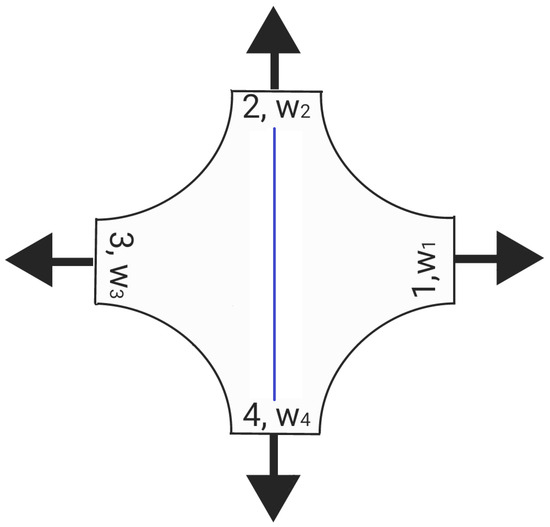
\includegraphics[width=0.3\linewidth]{img/malt_dirichlet.png}};
\node[boxL, below=8mm of fe, minimum width=46mm] (data) {Сбор данных\\ $D(p,w)=\{(C,S)\}$};

% MIDDLE COLUMN
\node[boxM, right=28mm of fe, minimum width=54mm] (xi) {деформация Лапласа\\ $\boldsymbol{\xi}=\boldsymbol{\xi}(C)$};
\node[boxM, below=8mm of xi, minimum width=54mm] (arch) {Архитектура CLaNN\\ $\psi_{\rm phys}(\boldsymbol{\xi})$};
\node[boxM, below=8mm of arch, minimum width=54mm] (smap) {Автодифференцирование \\ $S=\partial\psi/\partial C$};
\node[trainbox, below=8mm of smap, minimum width=54mm] (train) {Обучение\\ $L=\|\vect S_{pred}-\vect S\|_{L2}$ (Adam)};

% RIGHT COLUMN
\node[boxR, right=28mm of arch, minimum width=50mm] (gh) {Производные\\ $g(\xi),\ H(\xi)$};
\node[boxR, below=8mm of gh, minimum width=50mm, minimum height=36mm] (infl) {FE-раздутие\\ рексация + Ньютон\\[2pt]
  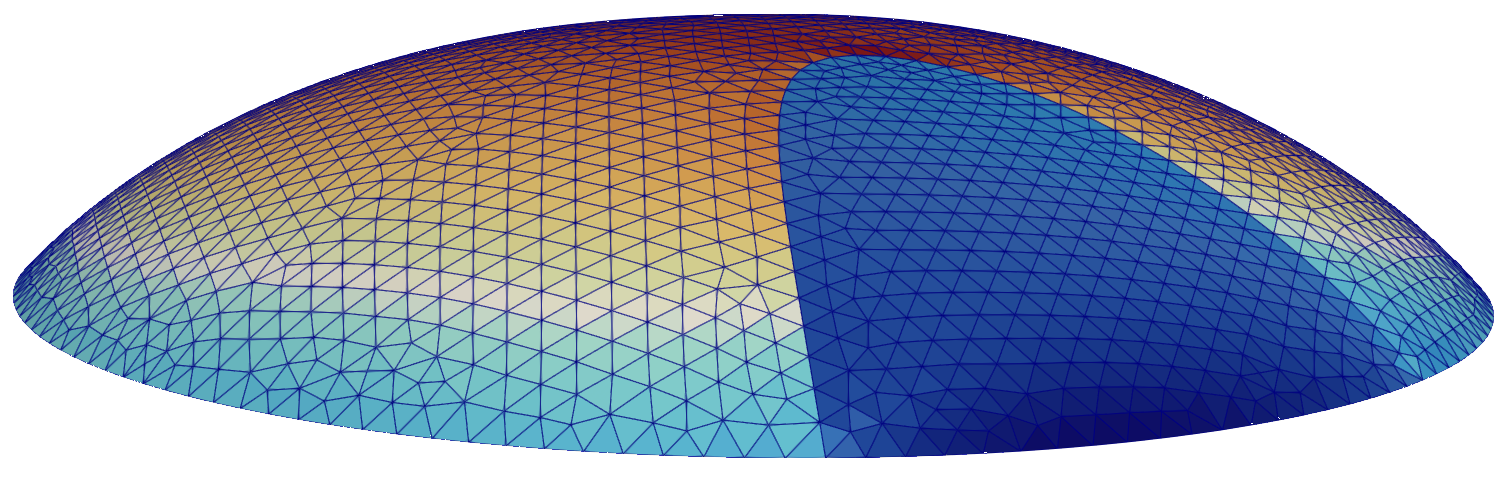
\includegraphics[width=0.3\linewidth]{img/Numerical/het/plane.png}};

% ORTHOGONAL ARROWS
\draw[->] (fe) -- (data);
% вилка от датасета: одна ветвь к деформации, другая — к обучению
\path (data.east) -- ++(10mm,0) coordinate (datasplit);
\draw[->] (data.east) -- (datasplit) |- (xi.west);
\draw[->] (datasplit) |- (train.west);
\draw[->] (xi) -- (arch);
\draw[->] (arch) -- (smap);
\draw[->] (smap) -- (train);
\draw[->] (arch.east) -- (gh.west);
\draw[->] (gh.south) -- (infl.north);
% пунктир: обновление параметров из обучения обратно в архитектуру (слева)
\draw[dashedarrow] (train.west) -- ++(-8mm,0) |- (arch.west);

\end{tikzpicture}
}
  \caption{Схема вычислительного контура CLaNN.}
  \label{fig:clann_pipeline}
\end{figure}

Такое построение архитектуры CLaNN обеспечивает выполнение всех необходимых физических свойств гиперупругой модели: 
\textbf{термодинамическая корректность} достигается через строгое соблюдение соотношения \eqref{eq:chain-rule}, 
что гарантирует консервативность напряжений $\oint \vect{S}:\mathrm{d}\vect{C} = 0$ и согласованность с законами 
термодинамики; 
\textbf{материальная устойчивость} обеспечивается и существенно улучшается за счёт строгой выпуклости функции энергии 
$\psi(\boldsymbol{\xi})$, гарантируемой архитектурой ICNN ($\vect{W}_2 \ge 0$, выпуклая неубывающая активация); 
\textbf{объективность} автоматически выполняется благодаря параметризации через тензор 
Коши-Грина $\vect{C} = \vect{F}^{\top}\vect{F}$, обеспечивая инвариантность относительно поворотов и симметрию напряжений; 
\textbf{строгая неотрицательность и коэрцитивность энергии} обеспечиваются архитектурной калибровкой 
$\psi_{\mathrm{phys}}(\boldsymbol{\xi}) = \mathbf{W}_2^{\top}(z - z_0) - \mathbf{r}_0^{\top}\boldsymbol{\xi}$,
что даёт $\psi_{\mathrm{phys}}(\mathbf{0})=0$, $\psi_{\mathrm{phys}}(\boldsymbol{\xi})>0$ при $\boldsymbol{\xi}\ne\mathbf{0}$ и 
$\psi_{\mathrm{phys}}(\boldsymbol{\xi})\to\infty$ при $\|\boldsymbol{\xi}\|\to\infty$; 
наконец, \textbf{физические ограничения} \eqref{eq:energy_constraints} обеспечиваются архитектурой сети CLaNN: монотонные, выпуклые функции активации,
неотрицательные весовые коэффициенты, центрирование энергии деформации $\psi$ и отклика $\vect r$.




% Virtual experiment / Results
\section{Virtual Experiment}
\section{Virtual experiment}

For training and testing CLaNN we used synthetic data of biaxial stretching and inflation of a hyperelastic membrane, respectively.
% Synthetic experimental data description removed in English build
Model training was performed on numerical experimental data, 
obtained for biaxial stretching of a specimen with a "Maltese cross" geometry and thickness $H=0.53$ mm (Figure \ref{fig:malt_geometry}) using the hyperelastic nodal force method \cite{ddaniso2024}. 
The membrane material was specified by a neo-Hookean model \cite{ogden1997nonlinear}:
\begin{align} \label{eq:neohook}
        \widetilde{\psi} &= \dfrac{\mu H(X)}{2} (I_1 +J^{-2}-3),
        \quad     I_1 = e^{2\xi_1} (1+\xi_3^2)+e^{2\xi_2},\quad J = e^{\xi_1+\xi_2}
\end{align}
with $\mu=0.43\cdot 10^6$ Pa.

% Details of data extraction across specimen regions (omitted)
% Equilibrium method is described in \cite{ddaniso2024}.

\begin{figure}[H]
  \centering
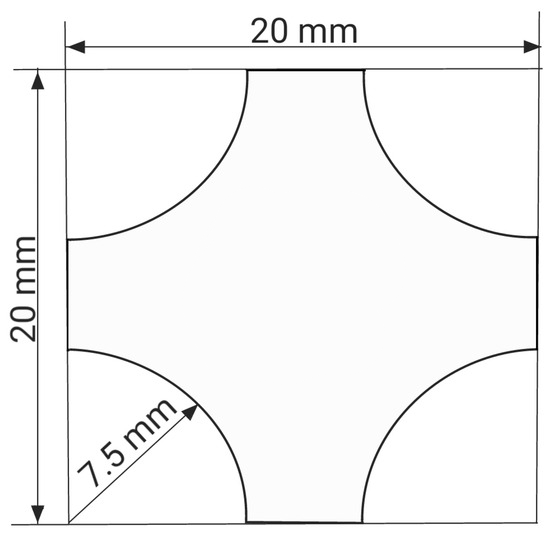
\includegraphics[width=0.4\textwidth]{../img/malt_geom.png}
\caption{Dimensions of the biomaterial specimen in the shape of a Maltese cross. 
  The cutout radius is the same for all notches}
  \label{fig:malt_geometry}
  \label{fig:malt_displacements}
\end{figure}

The specimen loading scheme is shown in Figure \ref{fig:malt_displacements}, where $w_i \in [0,1]$, $i \in \{1,4\}$
represents the fraction of the prescribed maximum displacement $u_{\max}$ for the $i$-th arm: $w_i = 0$ 
corresponds to a fixed arm, and $w_i = 1$ corresponds to the arm whose position was shifted and fixed at distance $u_{max}$. 
By varying $w_i$, different biaxial loading scenarios are obtained. 
In our virtual experiments we sequentially
displace the arms with increment $\Delta s$. 
The displacement $w_i \cdot n \cdot \Delta s$ is applied to the $i$-th arm at step $n$, where $n = 1, \ldots, N$, 
$N = u_{\max}/\Delta s$ is the number of steps. 
The hyperelastic nodal force method was applied to the initially flat quasi-uniform unstructured triangulation with mesh size $h=0.5$ mm and size $5\,404$ triangles. The maximum arm displacement
$u_{\max} = 2$ mm and $\Delta s = 0.2$ mm.
At each step, $\mathbb{C}, \mathbb{S}$ were extracted for all triangles belonging to the selected observation window. 
% Using linear (P1) elements, (C,S) are cellwise constants.

 
 
Our testing protocol comprises nine experiments:

\begin{figure}[H]
  \centering
  \begin{minipage}[t]{0.48\textwidth}
    \centering
    \vspace{0pt}
    \begin{tabular}{|c|c|c|c|c|}
    \hline
    \textbf{No.} & $w_1$ & $w_2$ & $w_3$ & $w_4$ \\
    \hline
    1 & 1 & 1 & 1 & 1 \\
    2 & 1 & 0.75 & 1 & 0.75 \\
    3 & 0.75 & 1 & 0.75 & 1 \\
    4 & 1 & 0.5 & 1 & 0.5 \\
    5 & 0.5 & 1 & 0.5 & 1 \\
    6 & 1 & 1/3 & 1 & 1/3 \\
    7 & 1/3 & 1 & 1/3 & 1 \\
    8 & 1 & 0 & 1& 0 \\
    9 & 0 & 1 & 0 & 1 \\
    \hline
    \end{tabular}
\captionof{table}{Test experiment protocols}
    \label{tab:test_protocols}
  \end{minipage}\hfill
  \begin{minipage}[t]{0.48\textwidth}
    \centering
    \vspace{0pt}
    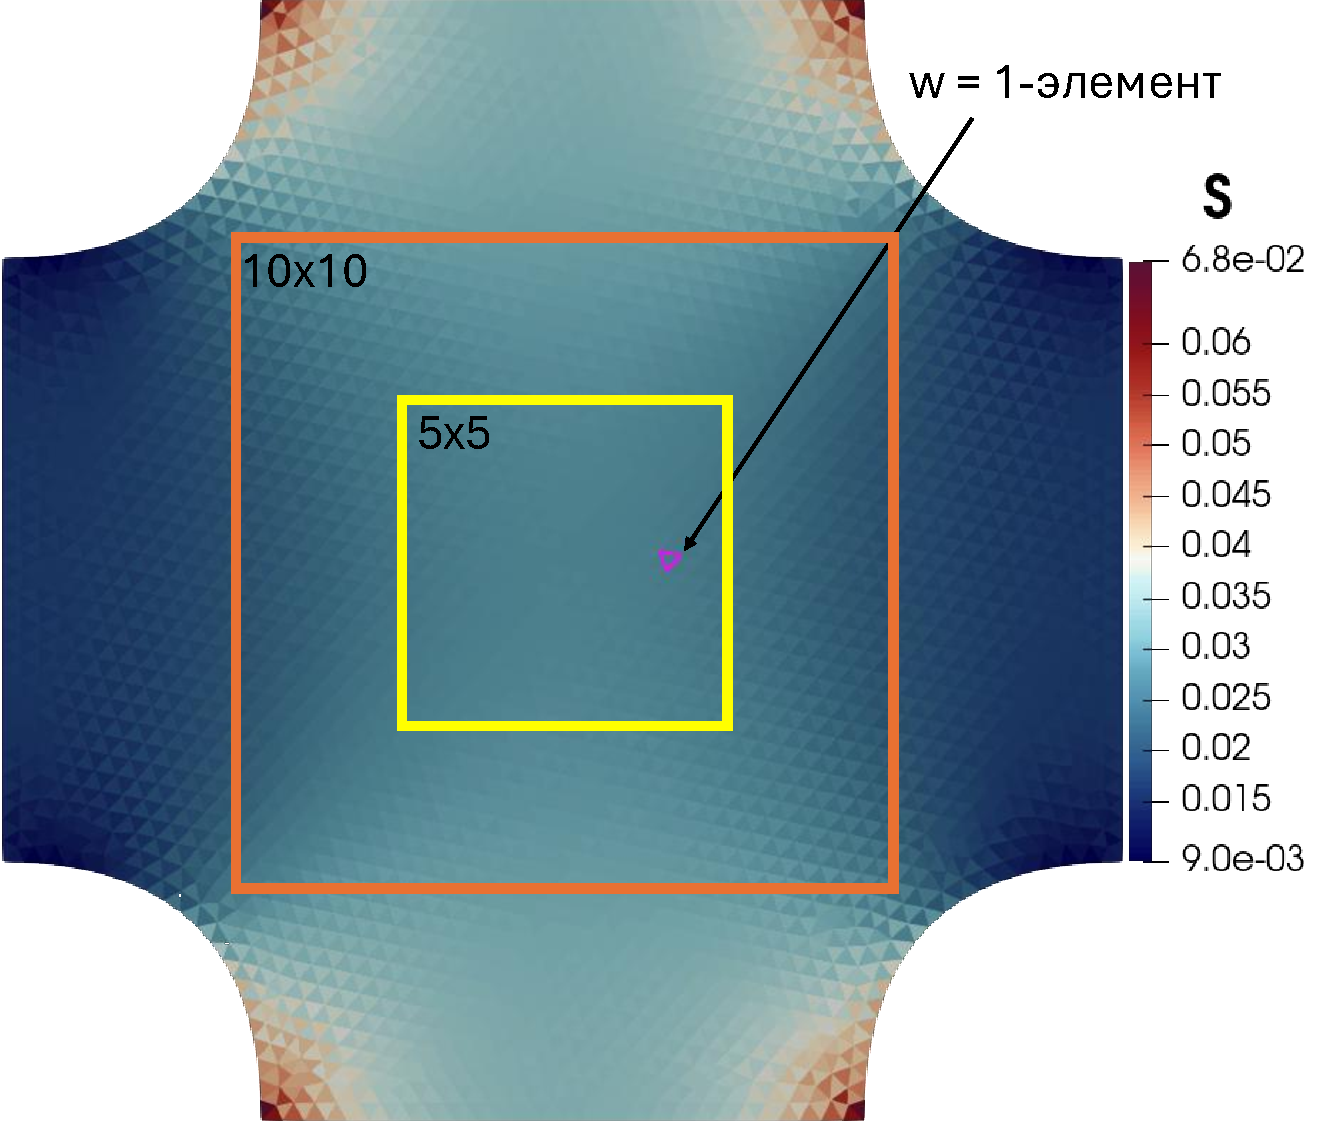
\includegraphics[width=\linewidth]{../img/Numerical/malt_window.pdf}
\captionof{figure}{Stress field $\vect S$ of the deformed membrane with "Maltese cross" geometry for different observation windows $w$.}
    \label{fig:malt_window}
  \end{minipage}
\end{figure}

\subsubsection{Data selection rules}
\paragraph{Central window $w$.}
The window is defined in the reference configuration $\Omega_0$ as the central region around the geometric center, aligned with the mesh axes. For $w=5\times5$ mm and $w=10\times10$ mm, we take squares of side 5 and 10 mm, respectively, centered at the specimen center; for $w=\text{full field}$ we take the entire $\Omega_0$. For $w=\text{1-element}$ we take the single central triangle (the minimal-index cell in the 5x5 mm window in $\Omega_0$ as shown in Figure~\ref{fig:malt_window}). Observations include all triangles whose barycenters $\mathbf{X}_T$ lie within the chosen window $\mathcal{W}_w\subset\Omega_0$.
% TODO: window cardinality in cells

\paragraph{Composition of observations (data).}
At each load step $n=1,\dots,N$ and for each triangle $T\in\mathcal{T}_w$ (cells within the window) we record the pair $(\mathbb C_T^{(n)},\,\mathbb S_T^{(n)})$, where $\mathbb C$ is the right Cauchy--Green tensor and $\mathbb S$ is the PK2 stress. Units: window sizes in mm; $\mathbb C$ dimensionless; $\mathbb S$ in MPa. Typical counts: 1 ($w=\text{1-element}$), 252 ($5\times5$ mm), 954 ($10\times10$ mm), and 5404 (full field).

\paragraph{Dataset formation.}
For fixed $(p,w)$, the set of all pairs $(\mathbb C_T^{(n)},\,\mathbb S_T^{(n)})$ forms the base dataset $D(p,w)$, which is split into $D_{\mathrm{tr}}(p,w)$ and $D_{\mathrm{val}}(p,w)$. For protocols $p$ (Table~\ref{tab:test_protocols}) and windows $w\in\{\text{1-element},5\times5\,\text{mm},10\times10\,\text{mm},\text{full field}\}$, denote
\[
  D_{\mathrm{tr}}\equiv D_{\mathrm{tr}}(p,w),\qquad D_{\mathrm{val}}\equiv D_{\mathrm{val}}(p,w),
\]
where $D_{\mathrm{tr}}$ is the training set and $D_{\mathrm{val}}$ is the validation set.

For example, $|D(\{1..10\}, \text{1-element})|=90$ points of $(\mathbb C,\mathbb S)$ (Figure \ref{fig:training_data}).

\begin{figure}[H]
  \centering
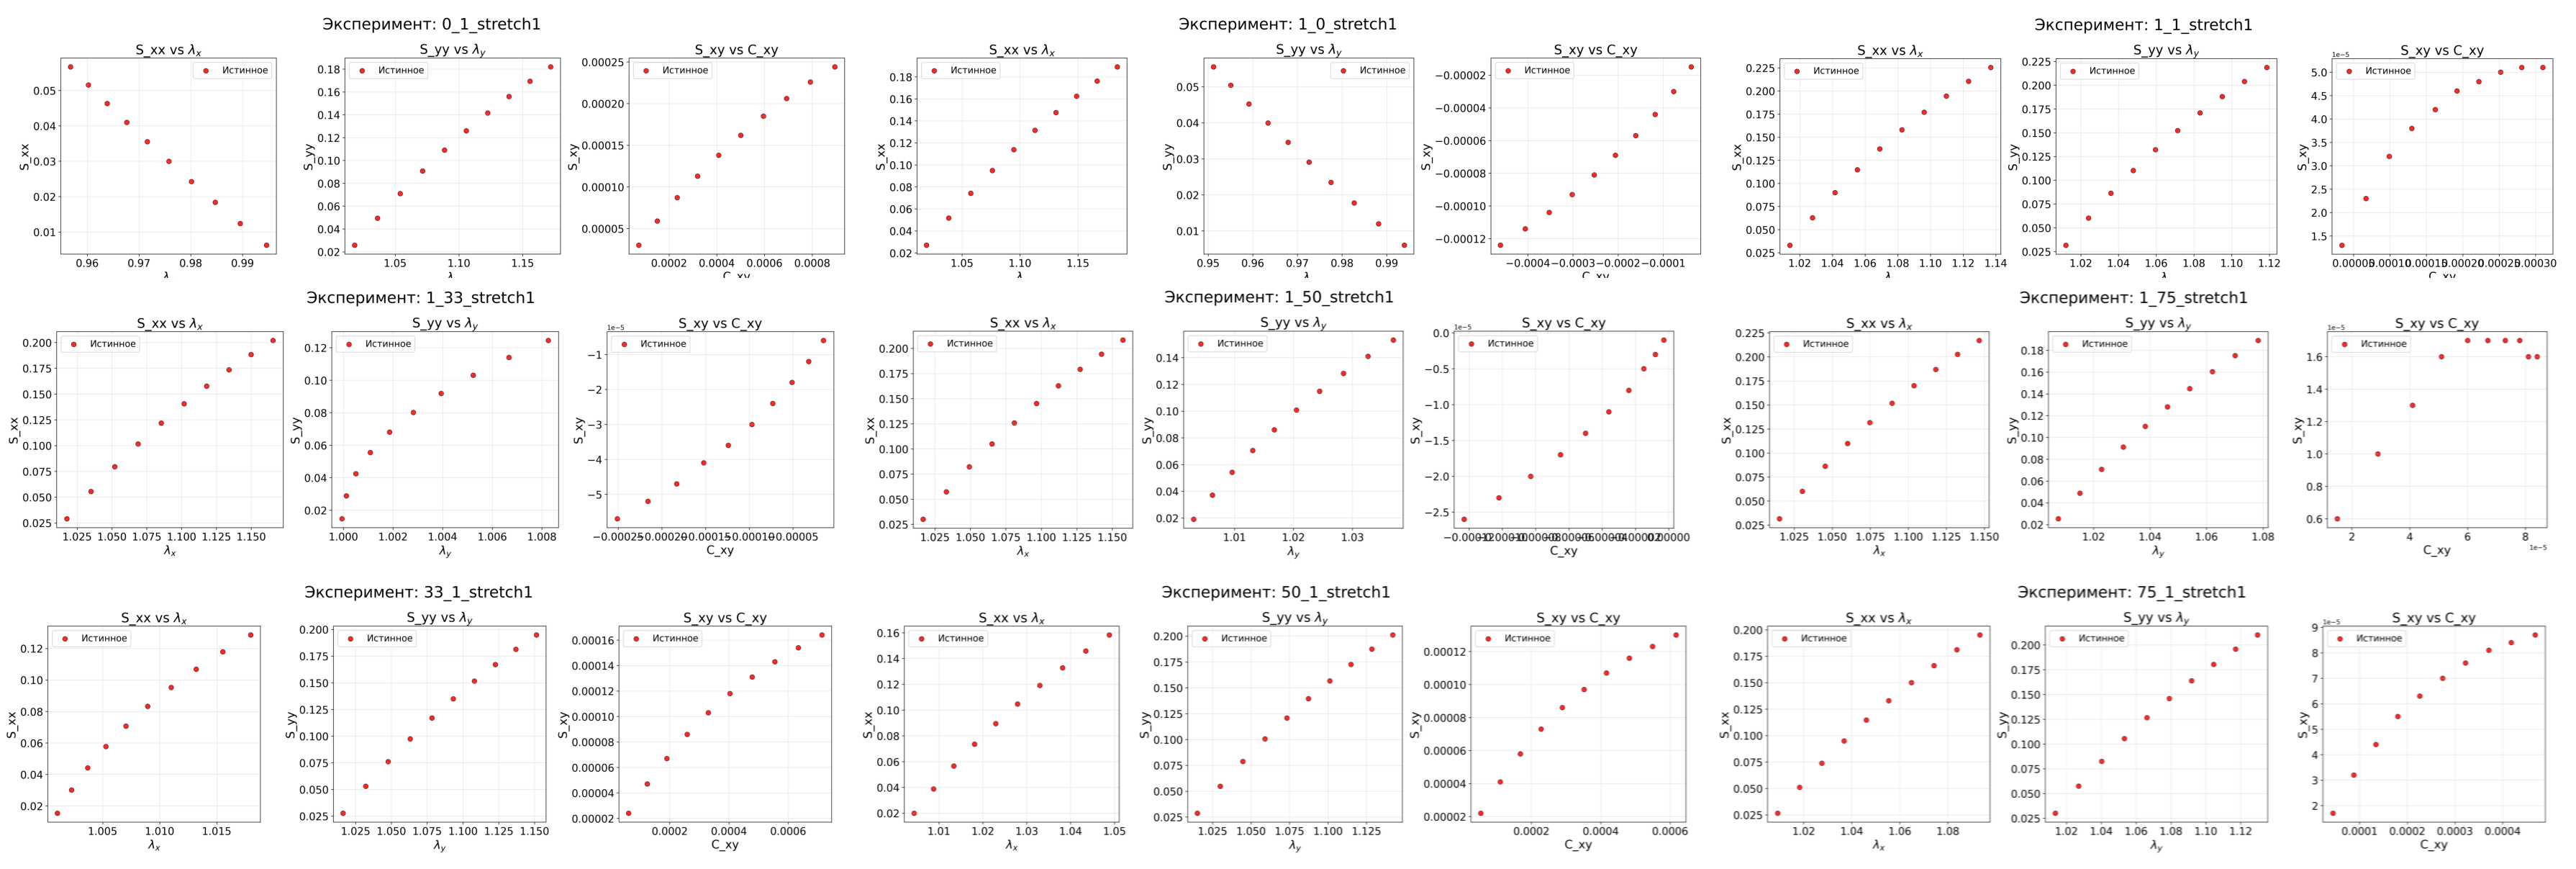
\includegraphics[width=1.0\textwidth]{../img/all_stress_plots.png}
\caption{Training dataset}
  \label{fig:training_data}
\end{figure}

Because data from a single central mesh element produce axial components much larger than shear ($2$--$3$ orders), expanding $w$ improves shear observability.

\subsubsection{Metrics and quality criteria}
\label{sec:metrics}

We use integral and pointwise metrics consistent with variational elasticity norms (e.g., \cite{ciarlet1988mathematical,ogden1997nonlinear,holzapfel2000nonlinear}).

\textbf{Coefficient of determination $R^2$.}
\begin{equation}\label{eq:r_squared}
  R^2 = 1 - \frac{\sum_{i=1}^n (y_i - \hat{y}_i)^2}{\sum_{i=1}^n (y_i - \bar{y})^2},
\end{equation}
where $y_i$ are experimental values, $\hat{y}_i$ are model predictions, $\bar{y}$ is the mean, and $n$ is the number of points.

\textbf{Pointwise relative error.}
\begin{equation}\label{eq:rel_error}
  \epsilon = \frac{\| \mathbb S - \mathbb S_{\text{ref}} \|}{\| \mathbb S_{\text{ref}} \|}.
\end{equation}
% purpose: plot error-field structure

\textbf{P1 error} \cite{xie2024p1} — a combination of absolute and relative errors, sensitive to small values:
\begin{equation}\label{eq:p1_error}
  \epsilon_{\mathrm{P1}} = \frac{\| \mathbb S - \mathbb S_{\text{ref}} \|}{s_0 + \| \mathbb S_{\text{ref}} \|},\qquad s_0 = \max(\mathbb S_{\text{pred}}).
\end{equation}

\textbf{Absolute integral error (mesh L2) for stresses (Frobenius norm).}
\begin{equation}\label{eq:l2_abs_stress}
  \|e\|_{L^2} = \Bigg( \sum_{K} \overline{\| \mathbb S_{\text{ref}} - \mathbb S_{\text{pred}} \|_F^{2}}^{\,K}\, |K| \Bigg)^{\tfrac12},
\end{equation}
where $|K|$ is the cell measure (area). For cell data, no intra-cell averaging is required:
\begin{equation}\label{eq:l2_abs_stress_cell}
  \|e\|_{L^2} = \Bigg( \sum_{K} \| \mathbb S_{\text{ref},K} - \mathbb S_{\text{pred},K} \|_F^{2}\, |K| \Bigg)^{\tfrac12}.
\end{equation}
Purpose: collapses the error field into a scalar and is invariant to mesh refinement \cite{BrennerScott2008,AinsworthOden2000,Verfurth2013}.

\textbf{Relative integral error.}
\begin{equation}\label{eq:l2_rel_stress}
  \|e\|_{L^2,\,\mathrm{rel}}\;=\; \frac{\Big( \sum\limits_{K} 
  \| \mathbb S_{\mathrm{ref},K} - \mathbb S_{\mathrm{pred},K} \|_F^{2}\, |K| \Big)^{\tfrac12}}
  {\Big( \sum\limits_{K} \| \mathbb S_{\mathrm{ref},K} \|_F^{2}\, |K| \Big)^{\tfrac12}}\,.
\end{equation}
% purpose: proper comparison across stress levels


\textbf{Optimization hyperparameters:}
\begin{itemize}
  \item Learning rate: $0.001$
  \item Batch size: $4$ (90-point set) and $128$ (other sets)
  % \item Physics weights: $\lambda_{\text{SI}} = 0.1$, $\lambda_{\psi} = 0.1$
  \item Architecture: 16 hidden neurons
  \item Smoothing parameter $\beta$: $10$
\end{itemize}

\textbf{Training results:}
Optimization reduces loss by five orders within $<5000$ epochs (Figure~\ref{fig:loss_curve}), reflecting both architectural suitability and hyperparameter choice; strict convexity ensures a unique minimum and avoids local traps.

\begin{figure}[H]
  \centering
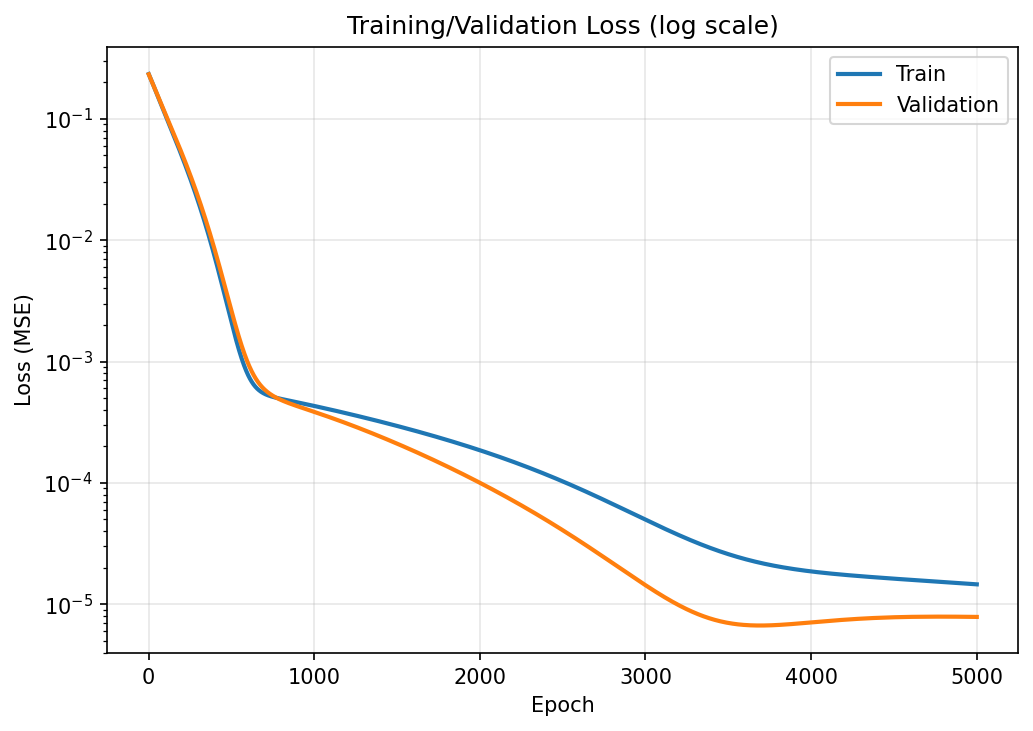
\includegraphics[width=0.7\textwidth]{../img/loss_curve.png}
  \caption{Loss curve when training on 90 data points}
  \label{fig:loss_curve}
\end{figure}


\subsection{Interpolation and extrapolation of loading curves}
We evaluate on $D_{\mathrm{tr}}(p,w)$ and $D_{\mathrm{val}}(p,w)$ at fixed $w$. We track $R^2_{\alpha}$, $\alpha\in\{xx,yy,xy\}$.

\textbf{Interpolation.}
Using 10 load levels from equi-biaxial ($p=1$), window $w=\text{1-element}$. CLANN achieves $R^2_{xx}=0.999$, $R^2_{yy}=0.999$, while $R^2_{xy}=0$ (Figure \ref{fig:interpolation}).

  \begin{figure}[H]
    \centering
    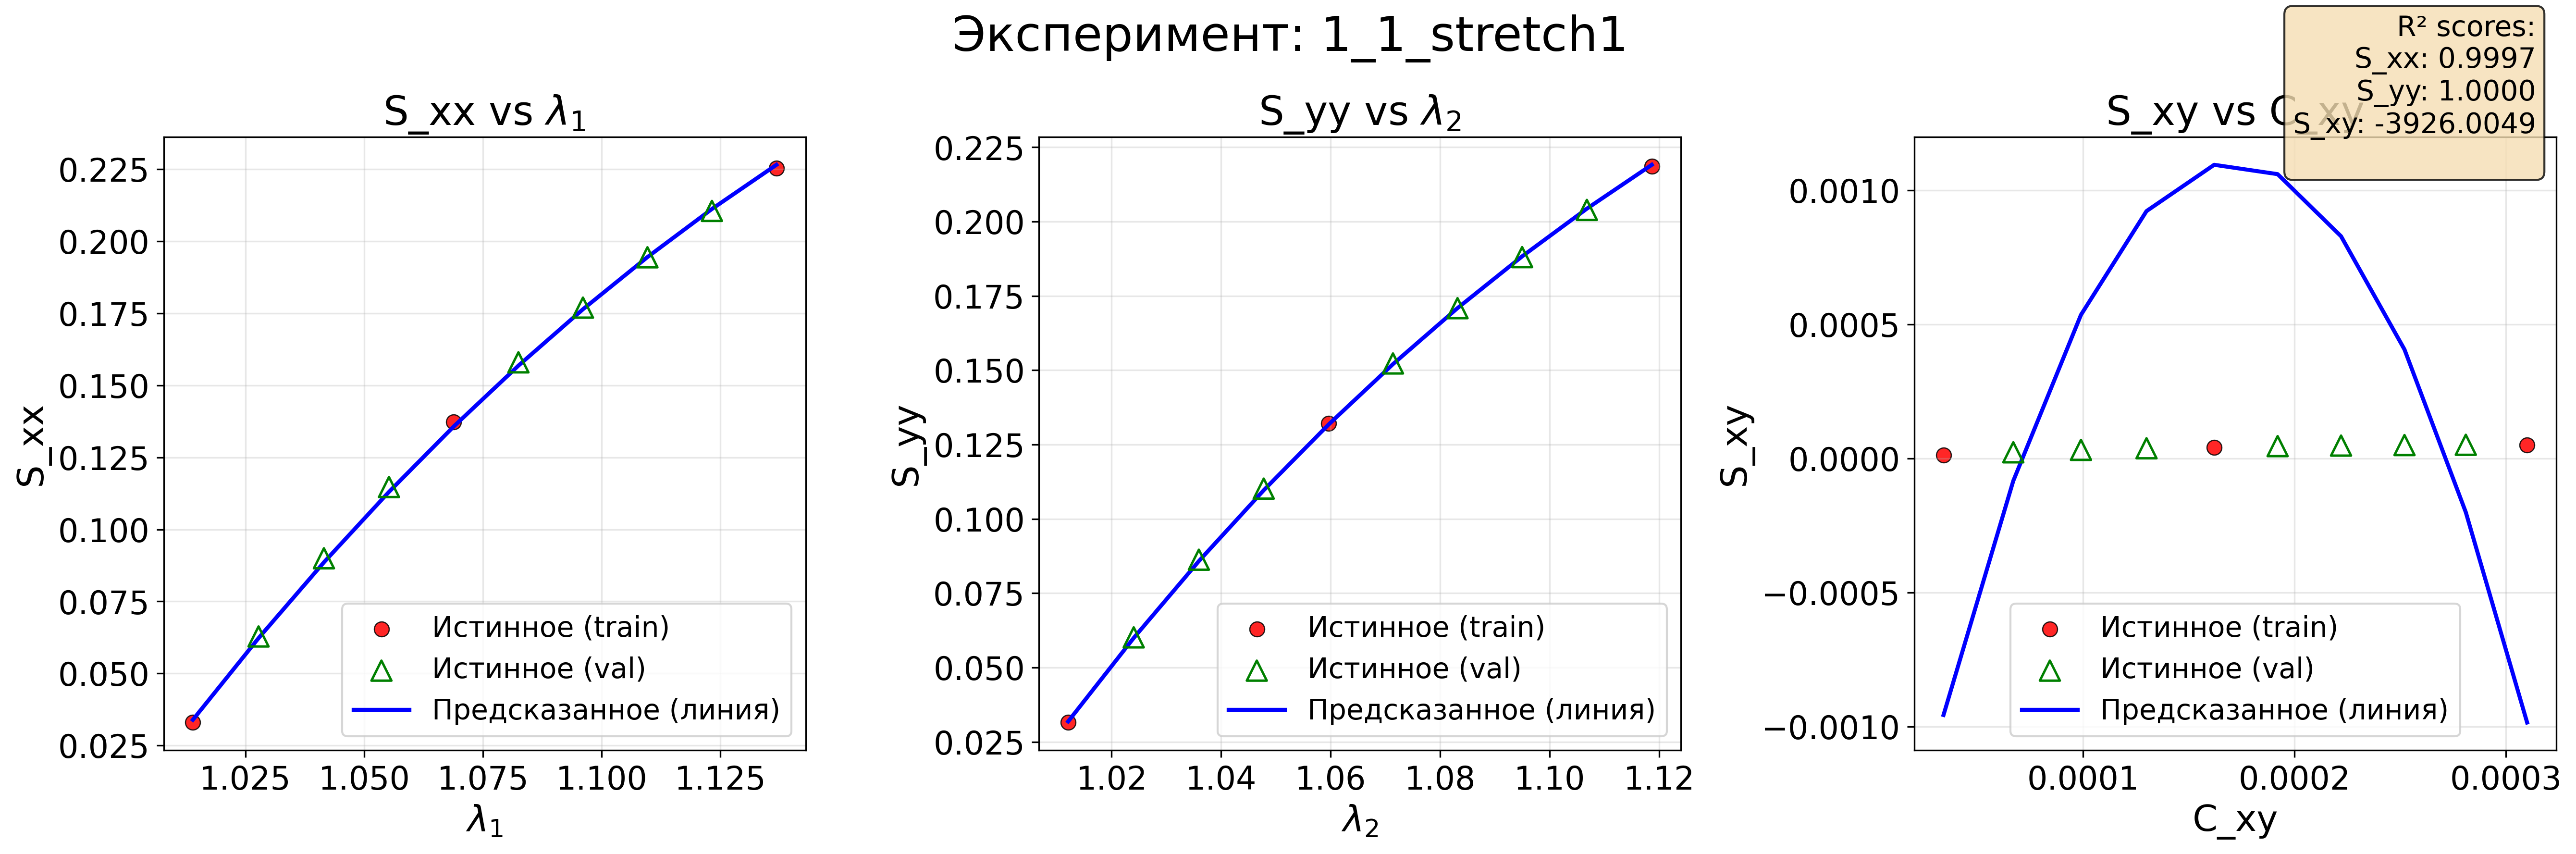
\includegraphics[width=1.0\textwidth]{../img/interpolation.png}
    \caption{Loading curve for equi-biaxial stretching}
    \label{fig:interpolation}
  \end{figure}
  
  \textbf{Extrapolation.}
  Train on $p=1$, validate on $p=9$, window $w=\text{1-element}$: $R^2_{xx}=0.993$, $R^2_{yy}=1.0$, $R^2_{xy}=0$ (Figure \ref{fig:extrapolation}).

  \begin{figure}[H]
    \centering
    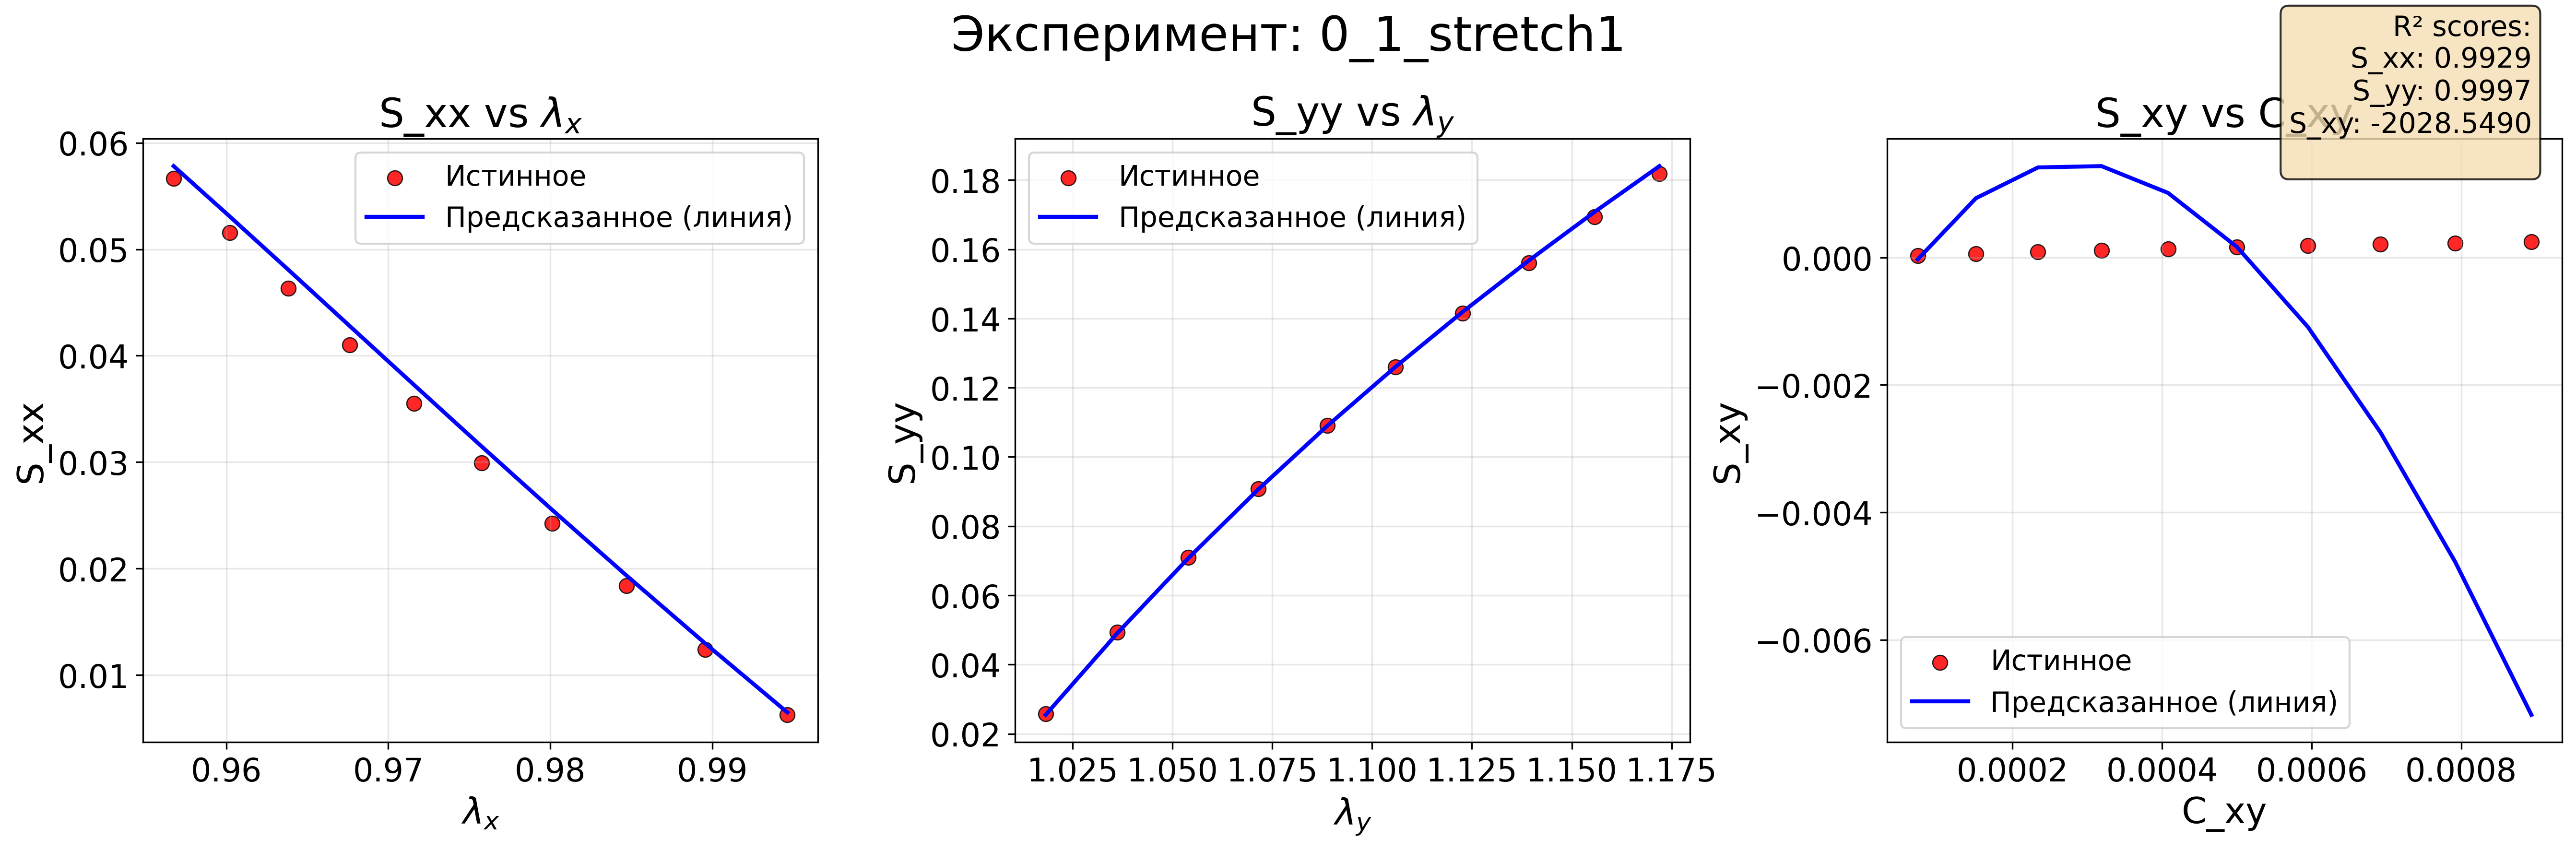
\includegraphics[width=1.0\textwidth]{../img/extrapolation.png}
    \caption{Loading curve for non-equi-biaxial stretching}
    \label{fig:extrapolation}
  \end{figure}
   
  Thus, CLANN interpolates and extrapolates axial components with high accuracy; shear prediction remains limited without richer shear coverage.
\subsection{Membrane inflation}

  We test inflation of a clamped circular membrane (radius 25 mm) under 5 MPa pressure, comparing CLANN to a Neo-Hookean reference with the same shear parameter as used in training-data generation.
  
  Two thickness fields $T$ are used: homogeneous (0.54 mm) and heterogeneous (two parabolic sectors of 2 mm within a 0.54 mm membrane), see Figure~\ref{fig:membrane_thickness}.

  As pointwise metric we use relative error (Section \ref{sec:metrics}, Eq.~\ref{eq:rel_error}); for shear comparison — P1 error \cite{xie2024p1} (Eq.~\ref{eq:p1_error}).

  \begin{figure}[H]
    \centering
    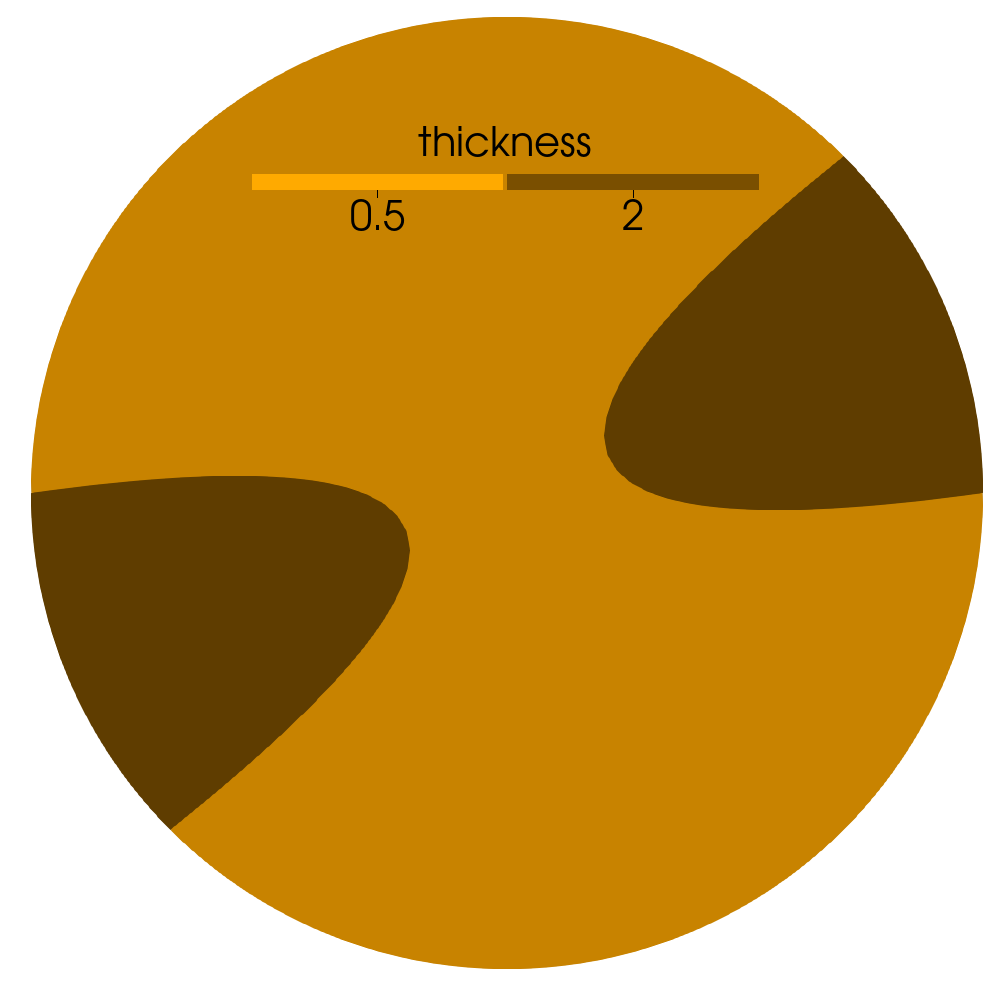
\includegraphics[width=0.25\linewidth]{../img/het_circle.png}
    \caption{Heterogeneous thickness field $T$ of the circular membrane.}
    \label{fig:membrane_thickness}
  \end{figure}

  \begin{figure}[H]
    \centering
    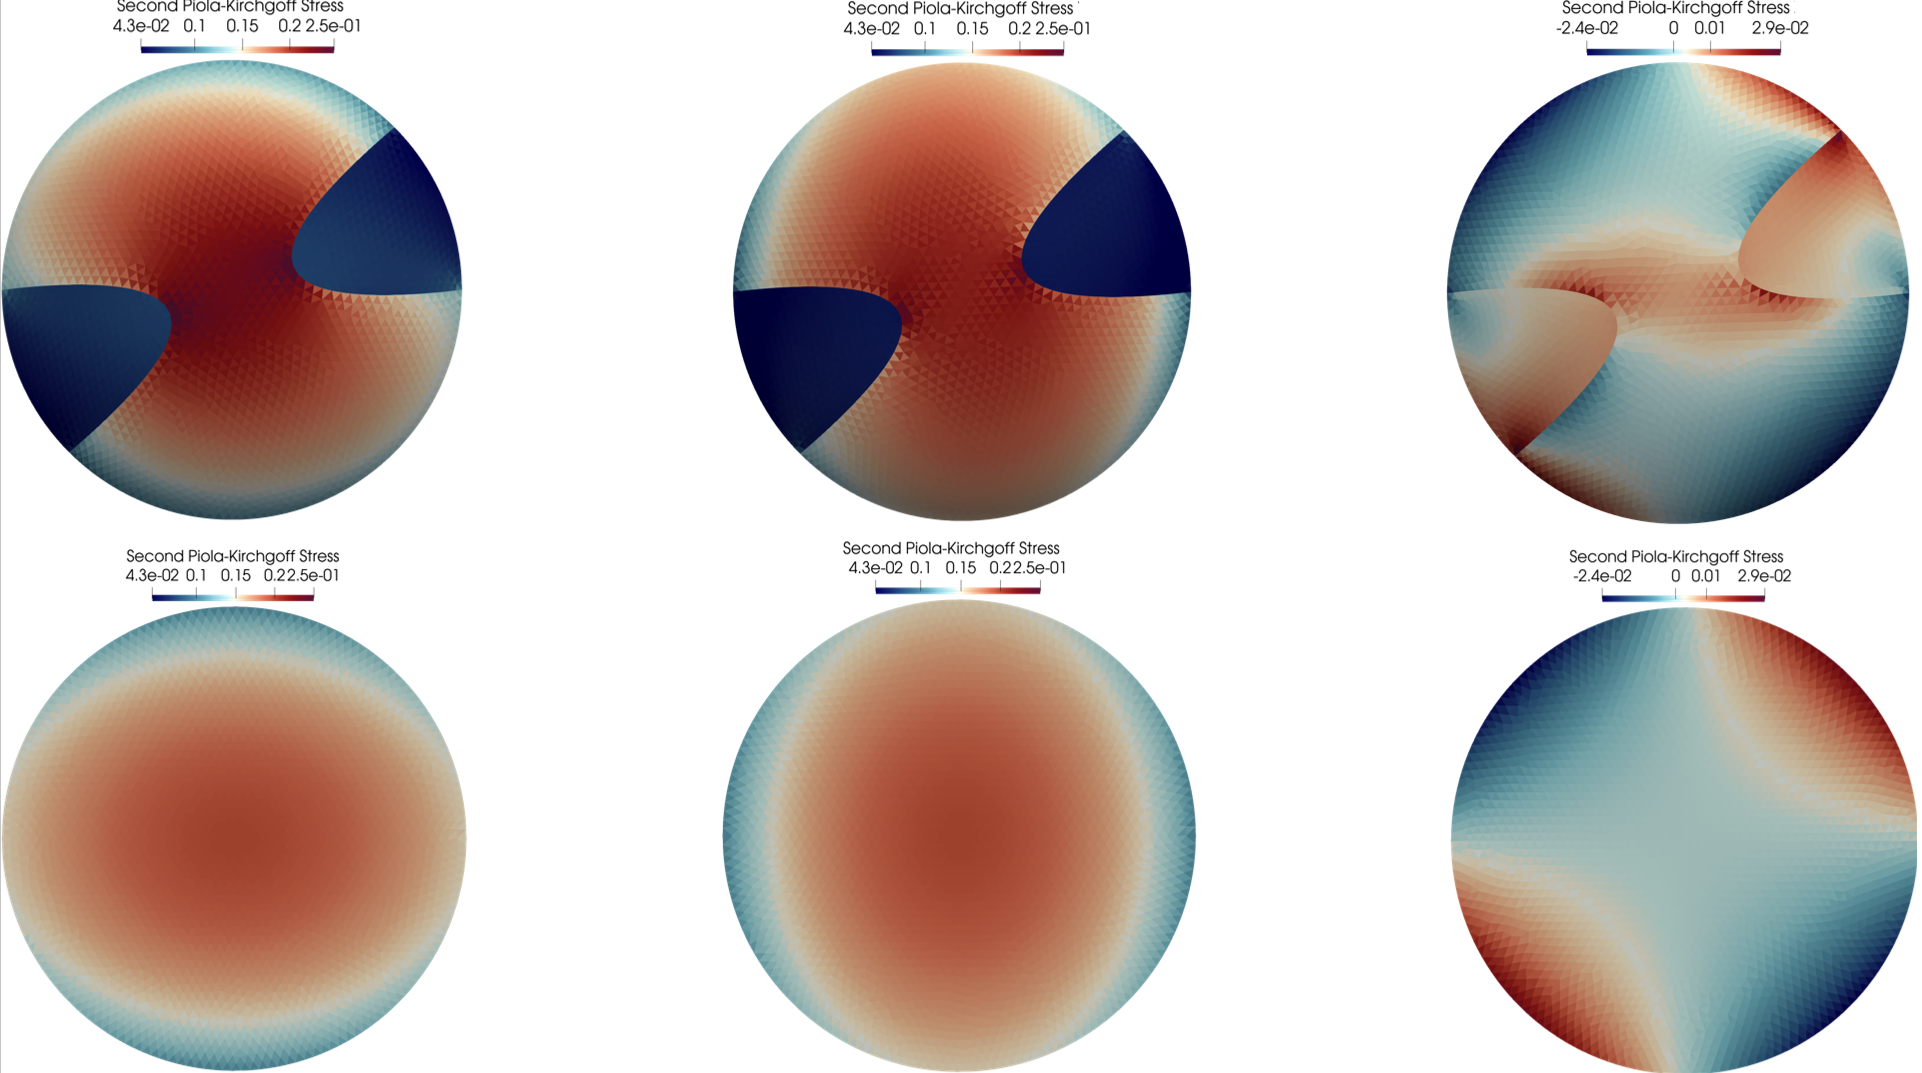
\includegraphics[width=0.7\textwidth]{../img/Numerical/ref_stress.png}
    \caption{PK2 stress field $\mathbb S$ of the circular membrane (example numerical result).}
    \label{fig:numerical_experiment}
  \end{figure}
  
  Using $D(\{1..10\}, w=\text{1-element})$ for training, we obtain PK2 stress fields for both thickness scenarios and compare to the reference (Figure~\ref{fig:membrane_thickness}, Figure~\ref{fig:inflation_ref}); error maps $\epsilon$ and $\epsilon_{P1}$ are shown in Figure~\ref{fig:numerical_errors}. Shear errors are largest for the heterogeneous case; expanding the window to $5\times 5$ mm, $10\times 10$ mm, and full field reduces integral errors $\|e\|_{L^2}$ (Eq.~\ref{eq:l2_abs_stress_cell}) and $\|e\|_{L^2,\,\mathrm{rel}}$ (Eq.~\ref{eq:l2_rel_stress}) (Figure~\ref{fig:integral_errors}).
  
  
  \begin{figure}[H]
    \centering
    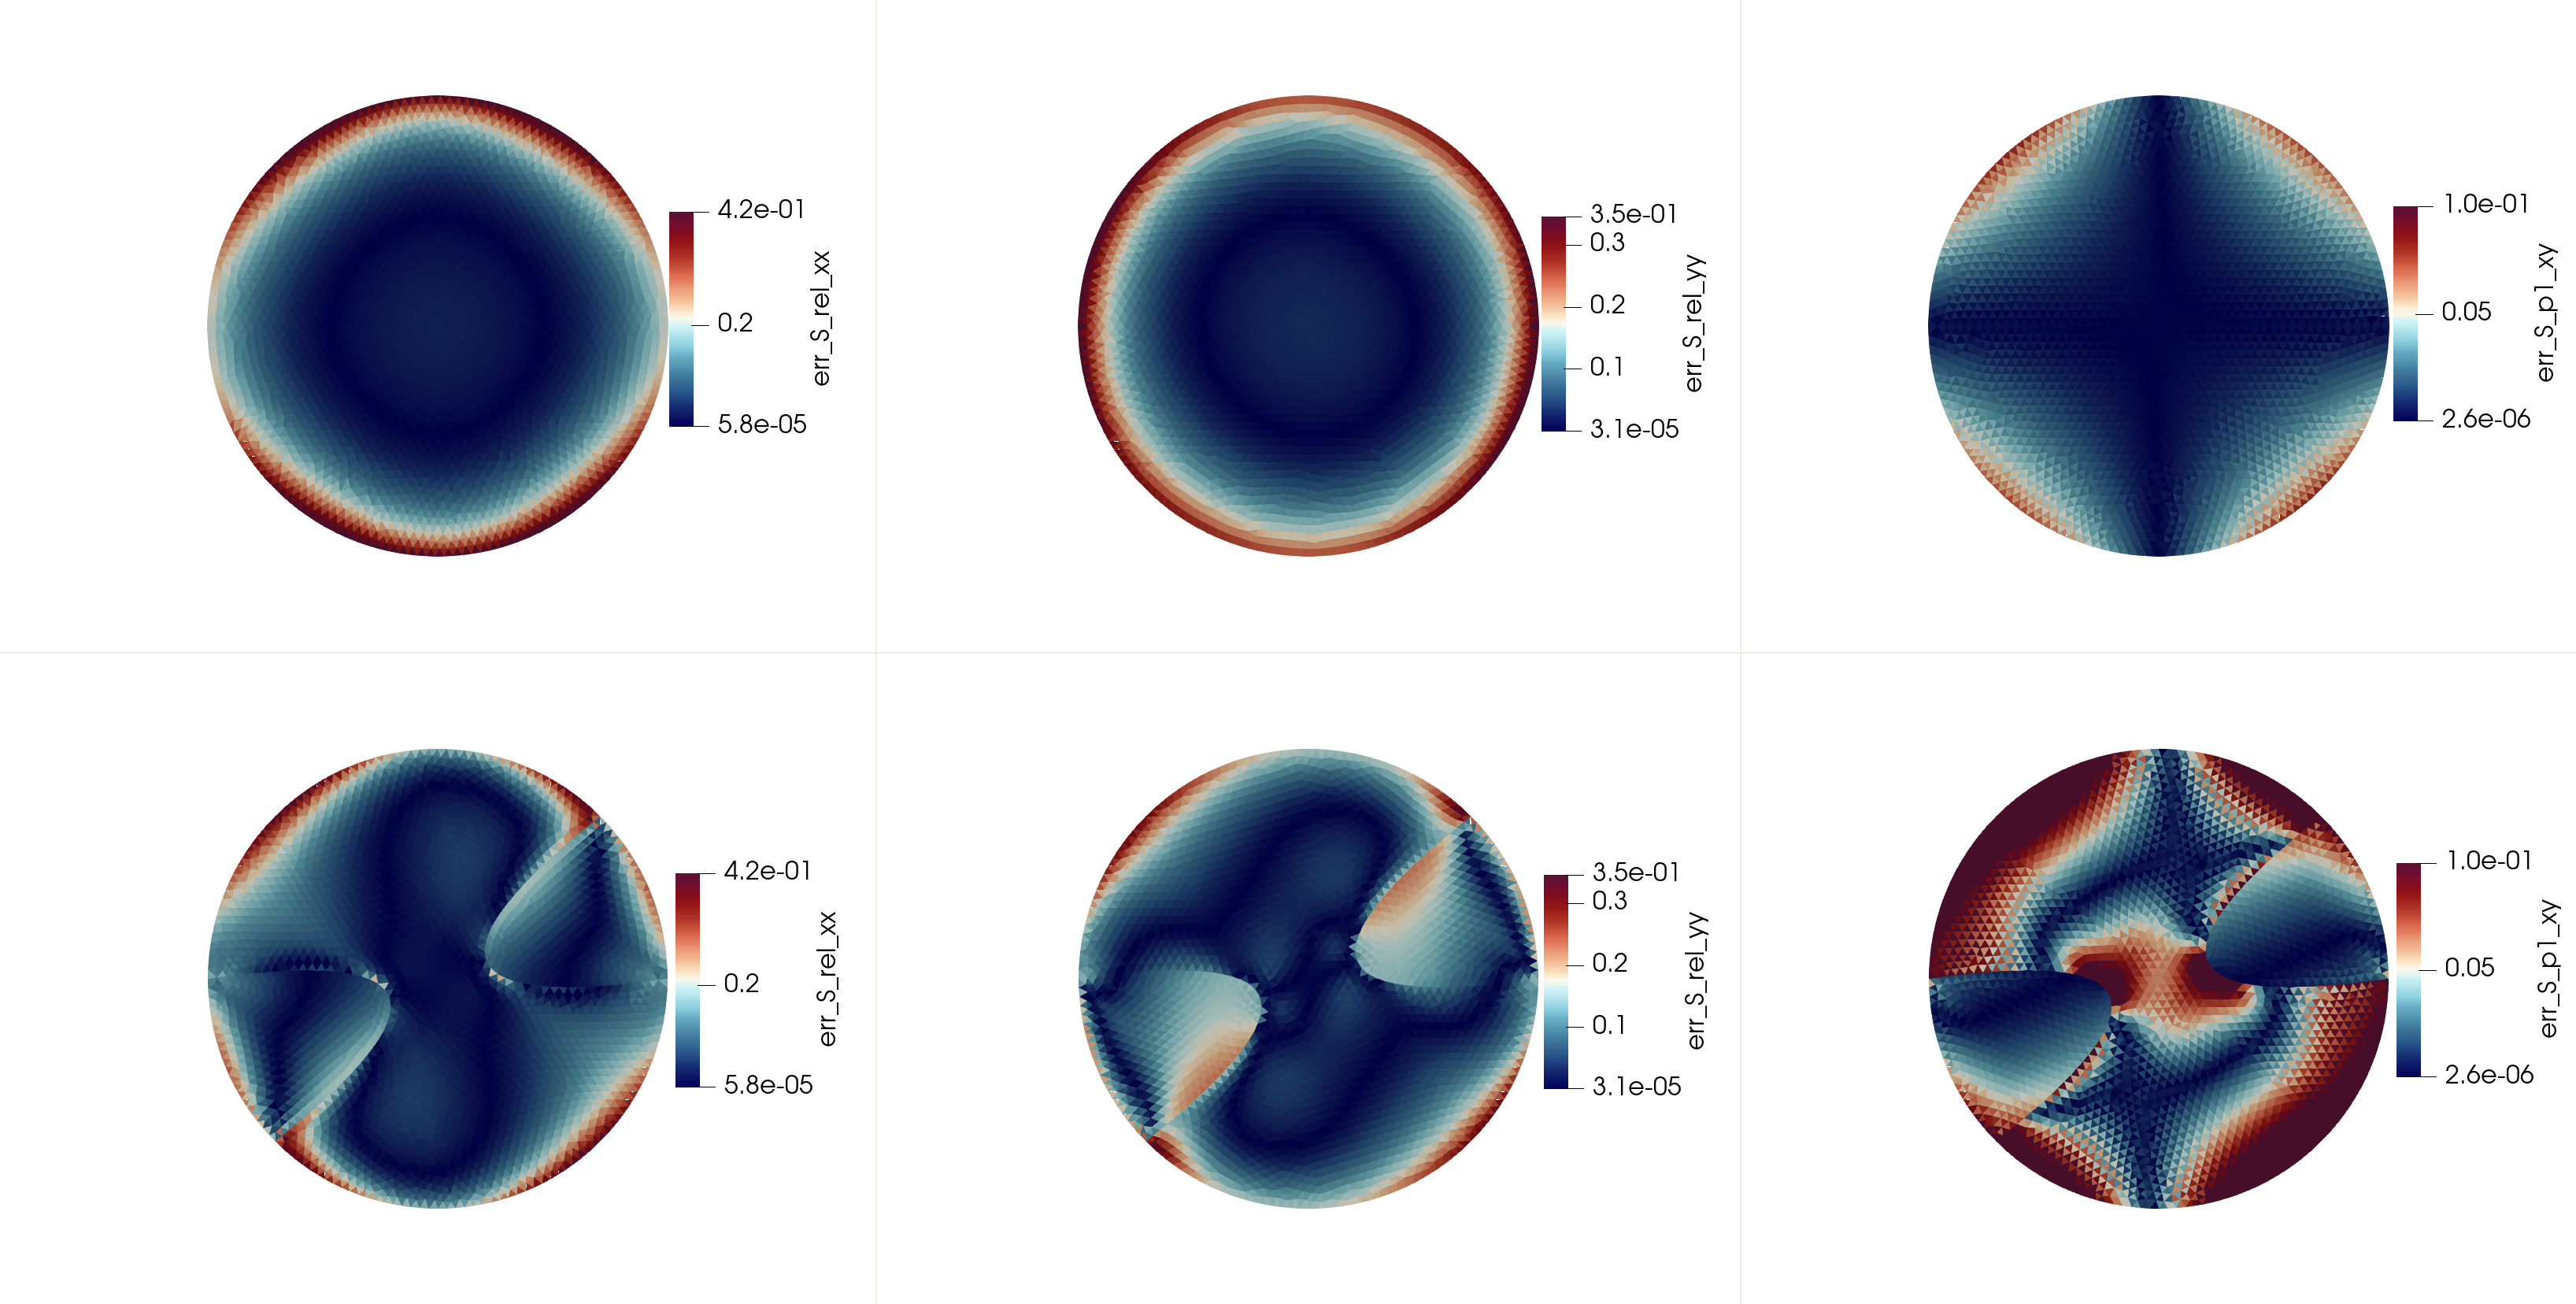
\includegraphics[width=1.0\textwidth]{../img/Numerical/errs.png}
    \caption{Error field between predicted and reference stresses.}
    \label{fig:numerical_errors}
  \end{figure}

  \begin{figure}[H]
    \centering
    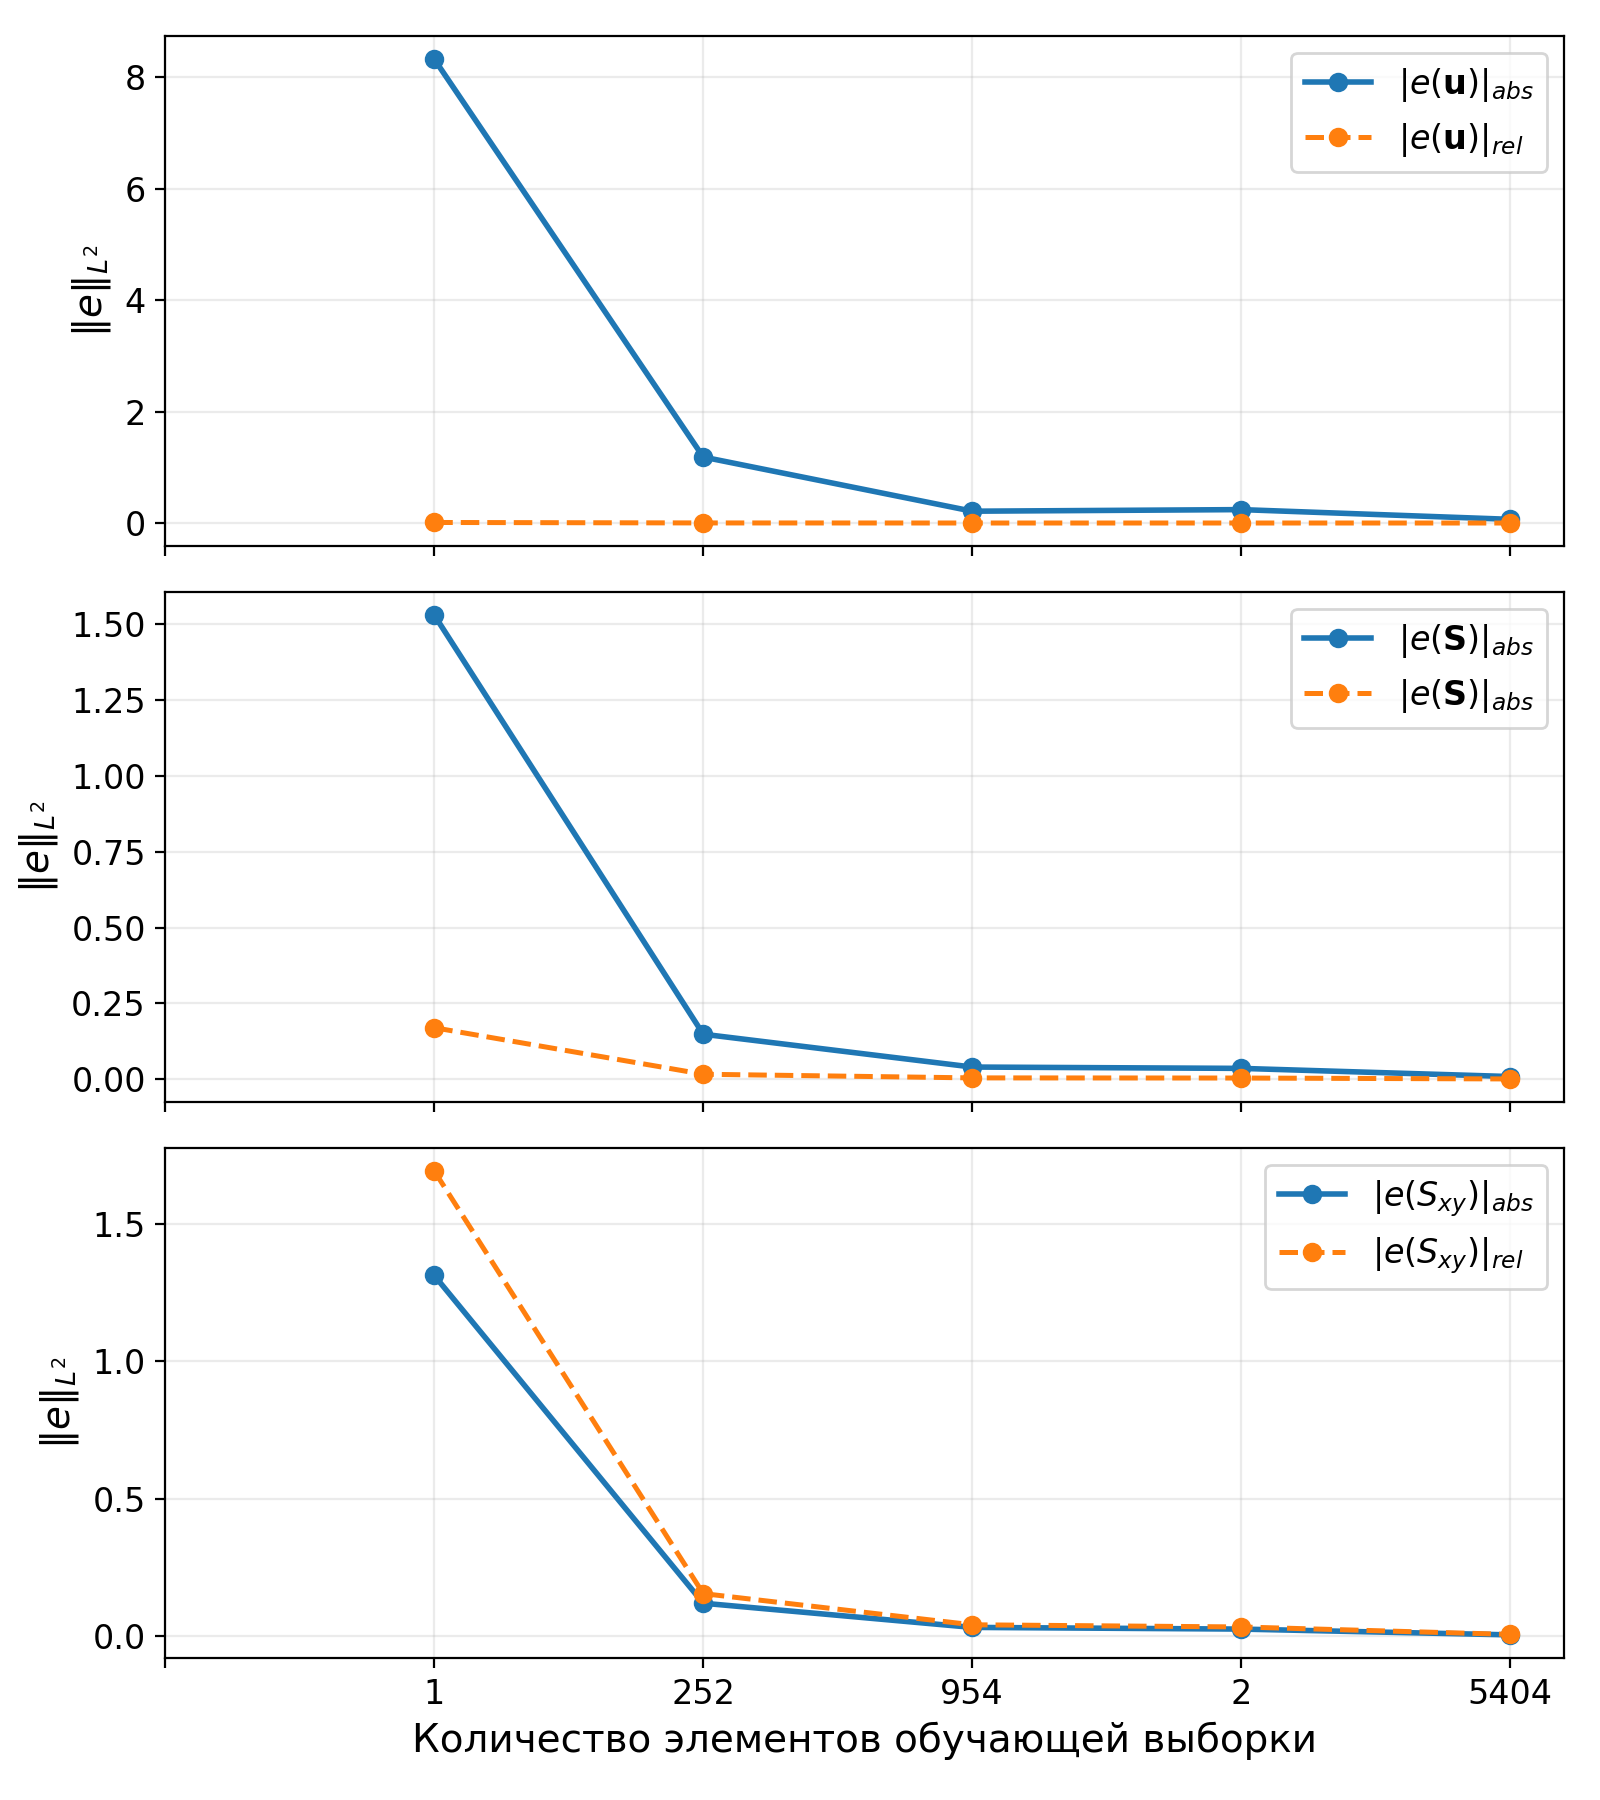
\includegraphics[width=0.5\textwidth]{../img/integral_errors.png}
    \caption{Integral errors $\|e\|_{L^2}$ and $\|e\|_{L^2,\,\mathrm{rel}}$ vs observation-window size $w$.}
    \label{fig:integral_errors}
  \end{figure}
  
  % integral errors vs window (omitted)
  
\subsection{Computational efficiency comparison}

  By strict convexity of $\psi(\boldsymbol\xi)$, the equilibrium is a smooth convex minimization amenable to gradient and Newton-type solvers with predictable complexity \cite{BoydVandenberghe2004,Nesterov2004,NocedalWright2006,ConnGouldToint2000}. Near the minimizer, strong convexity and Lipschitz Hessians yield locally quadratic Newton convergence, while L\textendash BFGS gives superlinear rates \cite{NocedalWright2006}.

  In tabulated/interpolatory DD models (kNN/IDW), energy convexity is typically not guaranteed and responses may be nonsmooth, yielding nonconvex optimization with many stationary points; quasi-static/relaxation strategies are used in practice \cite{KirchdoerferOrtiz2016,KirchdoerferOrtiz2017} at the cost of more load steps/iterations and repeated kNN/IDW queries.

  We compare runtime for CLANN, Neo-Hookean, and a Laplace-space table-driven DD model \cite{xi2023} on inflation of a clamped circular membrane ($R{=}25$ mm), with homogeneous and heterogeneous $T$ (Figure~\ref{fig:membrane_thickness}). CLANN is trained on $D(\{1..10\},\,w{=}\text{1-element})$; the DD model uses kNN/IDW on $(\vect{\xi},\vect r)$ from $D(\{1..10\},\,w{=}10\times10)$ \cite{xi2023}. All runs use the same FE setting and stopping criteria.

\begin{table}[htbp]
\centering
\caption{Runtime (s) for inflation: homogeneous vs heterogeneous thickness}
\label{tab:experiments_summary}
\begin{tabular}{|l|c|c|}
\hline
\textbf{Method} & \textbf{Homogeneous} & \textbf{Heterogeneous} \\
\hline
CLANN & 512 & 329  \\
\hline
Neo-Hooke & 13 & 16\\
\hline
kNN & 993 & -- \\
\hline
\end{tabular}
\end{table}

  With identical meshes and tolerances, CLANN matches Neo-Hooke in global iterations but can be slower overall due to model–solver interface overhead \cite{xi2023}. It notably outperforms the table-driven DD baseline by avoiding repeated kNN/IDW queries and data projections. The DD model further struggles on heterogeneous thickness without linear interpolation near zero, likely due to data scarcity in that strain range.




% Conclusions
\section{Conclusion}
\section{Conclusion}

We proposed a physics-informed CLaNN architecture for hyperelastic materials, based on a convex
strain energy potential and log\textendash Laplace kinematic parametrization.

The architecture ensures thermodynamic consistency; thanks to
convexity, the problem is solved as a smooth convex minimization with predictable convergence of gradient and
quasi-Newton methods.
At the same time, the architecture for stress computation does not explicitly use information about compressibility/incompressibility or isotropy/anisotropy
of the material, which allows CLaNN to be applied to problems with different material types.

In interpolation tests CLaNN achieves small errors given representative training data; in the extrapolation regime it maintains stability and physically plausible response,
whereas locally interpolatory DD models (k\textendash NN/IDW) exhibit artifacts outside the training window.

In numerical experiments of inflating a clamped circular membrane (homogeneous and heterogeneous thickness), CLaNN accurately
reproduces displacement and stress fields and exhibits fast, predictable convergence within a unified
FE formulation for all models compared.

In terms of computational efficiency, CLaNN outperforms the kNN\textendash based DD model: on the homogeneous case the gain is
about $\times 1.9$ due to the absence of costly k\textendash NN/IDW queries and external projections onto data at each iteration.
We note that the obtained speedup can be even higher with improved coupling between the solver and CLaNN, as well as optimal hyperparameter tuning.
For heterogeneous thickness CLaNN remains operational without special heuristics,
whereas the DD model requires additional regularization and/or data interpolation near small strains.
Also, the lack of a residual-based stopping criterion in relaxation methods for equilibrium problems can lead to a difficult-to-estimate increase in runtime
relative to Newton-type methods supported by CLaNN.

In summary, CLaNN combines mechanical soundness with the efficiency of neural networks: convex energy and differentiability provide stable 
solutions to variational problems and accelerate computation compared with classical DD approaches, and show high approximation capability for hyperelastic materials
on small datasets.
Future work: test anisotropic materials and real experimental data.




% Appendix
\appendixtitles{yes}
\appendixstart
\appendix
\appendix

\chapter{\texorpdfstring{Эквивалентность QR-факторизации $\vect F$ и разложения Холецкого $\vect C=\vect F^{\top}\vect F$ для вычисления логарифмических координат $\boldsymbol{\xi}$}{Эквивалентность QR и Холецкого}}
\label{app:cholesky}

\section{Постановка и обозначения}

Рассматривается двумерная гиперупругая кинематика. Пусть:
\begin{itemize}
  \item $\vect F \in \mathbb{R}^{2 \times 2}$ — градиент деформации, $\det \vect F > 0$,
  \item $\vect C = \vect F^{\top}\vect F$ — правый тензор Коши–Грина (симметричный положительно определённый, SPD),
  \item Холецкий: $\vect C = \vect U^{\top}\vect U$, где $\vect U$ — верхнетреугольная и $\text{diag}(\vect U) > 0$,
  \item Логарифмические координаты:
    $\boldsymbol{\xi} = (\xi_1, \xi_2, \xi_3) = (\ln u_{11}, \ln u_{22}, u_{12}/u_{11})$.
\end{itemize}

Цель: показать, что при наличии $\vect F$ можно заменить вычисление $\vect U = \text{chol}(\vect C)$ на $\vect U = \vect R$ из тонкого QR($\vect F$) = $\vect Q \vect R$ (с $\text{diag}(\vect R) > 0$), и получить те же $\boldsymbol{\xi}$.

\section{Теорема (эквивалентность U и R)}

Пусть $\vect F \in \mathbb{R}^{2 \times 2}$ невырождённая ($\det \vect F > 0$). Рассмотрим тонкую QR-факторизацию
\begin{equation}
\vect F = \vect Q \vect R,
\end{equation}
где $\vect Q \in \mathbb{R}^{2 \times 2}$ — ортогональная ($\vect Q^{\top}\vect Q = \vect I$), $\vect R \in \mathbb{R}^{2 \times 2}$ — верхнетреугольная. Выберем стандартную нормализацию $\text{diag}(\vect R) > 0$. Тогда $\vect R$ совпадает с фактором Холецкого для $\vect C$:
\begin{equation}
\vect R = \text{chol}(\vect C), \quad \text{с} \quad \vect C = \vect F^{\top}\vect F.
\end{equation}

\textbf{Доказательство.}
\begin{equation}
\vect C = \vect F^{\top}\vect F = (\vect Q \vect R)^{\top}(\vect Q \vect R) = \vect R^{\top} \vect Q^{\top} \vect Q \vect R = \vect R^{\top} \vect R.
\end{equation}
Так как $\vect C$ — SPD и $\vect R$ — верхнетреугольная с положительной диагональю, то представление $\vect C = \vect R^{\top}\vect R$ единственно. По единственности фактора Холецкого (с $\text{diag} > 0$) следует $\vect R = \text{chol}(\vect C)$. $\square$

\textbf{Следствие.} Логарифмические координаты $\boldsymbol{\xi}$, определённые через $\vect U = \text{chol}(\vect C)$, можно эквивалентно вычислять из $\vect U = \vect R$ в QR($\vect F$), при условии $\text{diag}(\vect R) > 0$.

\section{Координаты $\vect{\xi}$ через $\vect{U}$}

Для $\vect U = \begin{bmatrix} u_{11} & u_{12} \\ 0 & u_{22} \end{bmatrix}$, $\text{diag}(\vect U) > 0$,
\begin{equation}
\boldsymbol{\xi} = (\xi_1, \xi_2, \xi_3) = (\ln u_{11}, \ln u_{22}, u_{12}/u_{11}).
\end{equation}
Тем самым, $\boldsymbol{\xi}(\vect F) := \boldsymbol{\xi}(\vect R(\vect F)) = \boldsymbol{\xi}(\vect U(\vect C))$.




% Minimal references section placeholder
\reftitle{References}
\isAPAandChicago{}{\begin{thebibliography}{999}\bibitem[Author1(year)]{ref-journal}Author~1, T. The title of the cited article. {\em Journal Abbreviation} {\bf 2008}, {\em 10}, 142--149.\end{thebibliography}}

\end{document}


